\documentclass[11pt]{article}

\usepackage[T1]{fontenc}
\usepackage[utf8]{inputenc}
\usepackage{graphicx}
\usepackage[labelfont=bf]{caption}
\usepackage{booktabs, siunitx}
\usepackage{tikz}
\usepackage{tikz-qtree}
\usepackage{pifont}
\usepackage[margin=0.90in]{geometry}
\usepackage{etoolbox,titling}
\usepackage{enumitem}
\usepackage{fancyhdr}
\usepackage{soulutf8}
\usepackage{epigraph}
\usepackage{amssymb}
\usepackage[export]{adjustbox}
\usepackage{amsmath}
\usepackage[hidelinks]{hyperref}
\usepackage{hypcap}
\usepackage{textcomp}


\pagestyle{fancy}
\fancyhf{}
\rhead{Virginia Filippi e Chiara Solito}
\lhead{VaccineSupervision}
\rfoot{Pagina \thepage}
\lfoot{Bioinformatica - A.A. 2021/22}
\usetikzlibrary{trees}
\tikzstyle{every node}=[draw=black,thick,anchor=west]
\newcommand{\angstrom}{\mbox{\normalfont\AA}}

\begin{document}
\newcommand\tab[1][0.3cm]{\hspace*{#1}}


\begin{titlepage}
    \begin{center}
        \vspace*{1cm}
            
        \Huge
        \textbf{Vaccine Supervision}
            
        \vspace{0.5cm}
        \LARGE
        Progetto di Ingegneria del Software
            
        \vspace{2cm}
            
        \begin{tikzpicture}
            \clip (0,0.1) circle (2.55cm); \hspace*{-3.5cm}
            \node {
\includegraphics[scale=0.25]{pictures/VaccineSupervision.png}};
        \end{tikzpicture} 

        \vspace{2cm}

        \textbf{Virginia Filippi e Chiara Solito}

        \vspace{0.8cm}

        \Large
        Corso di Laurea in Bioinformatica\\
        Università degli studi di Verona\\
        A.A. 2021/22
            
    \end{center}
\end{titlepage}
La presente è la documentazione del progetto del corso di Ingegneria del Software, svolto nel contesto della laurea triennale in bioinformatica.\\
Insieme a questo documento in formato PDF viene fornito anche il codice \LaTeX  con cui è stato generato.
\tableofcontents
\thispagestyle{empty}

\newpage
    \section{Traccia dell'Elaborato}
    Riportiamo di seguito la traccia dell'elaborato:
        \begin{quotation}
            Si vuole progettare un sistema software per gestire le segnalazioni di reazioni avverse (ad esempio, asma, dermatiti, insufficienza renale, miocardiopatia, \dots) da vaccini anti-Covid.\\
            Ogni segnalazione è caratterizzata da un codice univoco, dall'indicazione del paziente a cui fa riferimento, dall'indicazione della reazione avversa, dalla data della reazione avversa, dalla data di segnalazione, e dalle vaccinazioni ricevute nei due mesi precedenti il momento della reazione avversa.
            Per ogni paziente sono memorizzati: un codice univoco, l'anno di nascita, la provincia di residenza e la professione.\\
            Per ogni paziente è possibile memorizzare gli eventuali fattori di rischio presenti (paziente fumatore, iperteso, sovrappeso, paziente fragile per precedenti patologie cardiovascolari o oncologiche), anche più d'uno. Ogni fattore di rischio è caratterizzato da un nome univoco, una descrizione e il livello di rischio associato. Per ogni paziente è, inoltre, memorizzata l'intera storia delle sue vaccinazioni precedenti, anti-Covid-19 e antinfluenzali.\\
            Ogni vaccinazione è caratterizzata da: paziente a cui si riferisce, segnalazioni a cui è legata, vaccino somministrato (AstraZeneca, Pfizer, Moderna, Sputnik, Sinovac, antinfluenzale, \dots), tipo della somministrazione (I, II, III o IV dose, dose unica), sede presso la quale è avvenuta la vaccinazione e data di vaccinazione. Per ogni reazione avversa sono memorizzati un nome univoco, un livello di gravità (da 1 a 5) e una descrizione generale, espressa in linguaggio naturale. Una reazione avversa può essere legata a molte segnalazioni. Per ogni paziente sono memorizzati il numero di reazioni avverse segnalate ed il numero di vaccinazioni ricevute.\\
            Il sistema deve supportare i medici che effettuano la segnalazione. Dopo opportuna autenticazione, il medico viene introdotto ad una interfaccia che permette l'inserimento dei dati delle reazioni avverse e dei pazienti. Il codice univoco dei pazienti è gestito dal sistema, che tiene traccia dei pazienti indicati da ogni medico. Ogni medico vede solo i codici identificativi dei pazienti, dei quali ha già segnalato qualche reazione avversa, e le relative informazioni.\\
            Ad ogni fine settimana o quando il numero di segnalazioni raggiunge la soglia di 50, il sistema manda un avviso ad uno dei farmacologi responsabili della gestione delle segnalazioni di reazioni avverse. Il farmacologo, dopo autenticazione, accede alle segnalazioni (tutte, con l'indicazione del medico che le ha fatte) e può effettuare alcune analisi di base (quante segnalazioni per vaccino, quante segnalazioni gravi in settimana, quante segnalazioni per provincia e quante segnalazioni per sede di vaccinazione).\\ Il sistema, inoltre, avvisa il farmacologo quando un vaccino ha accumulato in un mese oltre 5 segnalazioni di gravità superiore a 3.
            In base alle segnalazioni e agli avvisi del sistema, il farmacologo può proporre di attivare una fase di controllo del vaccino. Tale proposta viene registrata dal sistema, che tiene traccia di tutte le proposte relative ai vaccini segnalati.
        \end{quotation}
    \section{Analisi e Specifica dei Requisiti}
        \subsection{Specifiche casi d'uso}
        In questa sezione definiamo le proprietà dell'applicazione.\\
        Come dichiarato nella traccia il sistema prevede l'utilizzo da parte di due tipologie di personale medico: Medico e Farmacologo. 
        Entrambi i tipi di utente possono utilizzare l'applicazione dopo opportuno login: in questa sede si è previsto che gli utenti siano pre-registrati da un amministratore di sistema esterno (sul modello di sistemi medici già noti). Non è stato quindi previsto un form di registrazione, durante lo sviluppo e si suppone che ogni utente abbia a disposizione \texttt{username} e \texttt{password}.

        \paragraph*{Casi d'uso relativi al Medico}
            \begin{center}
                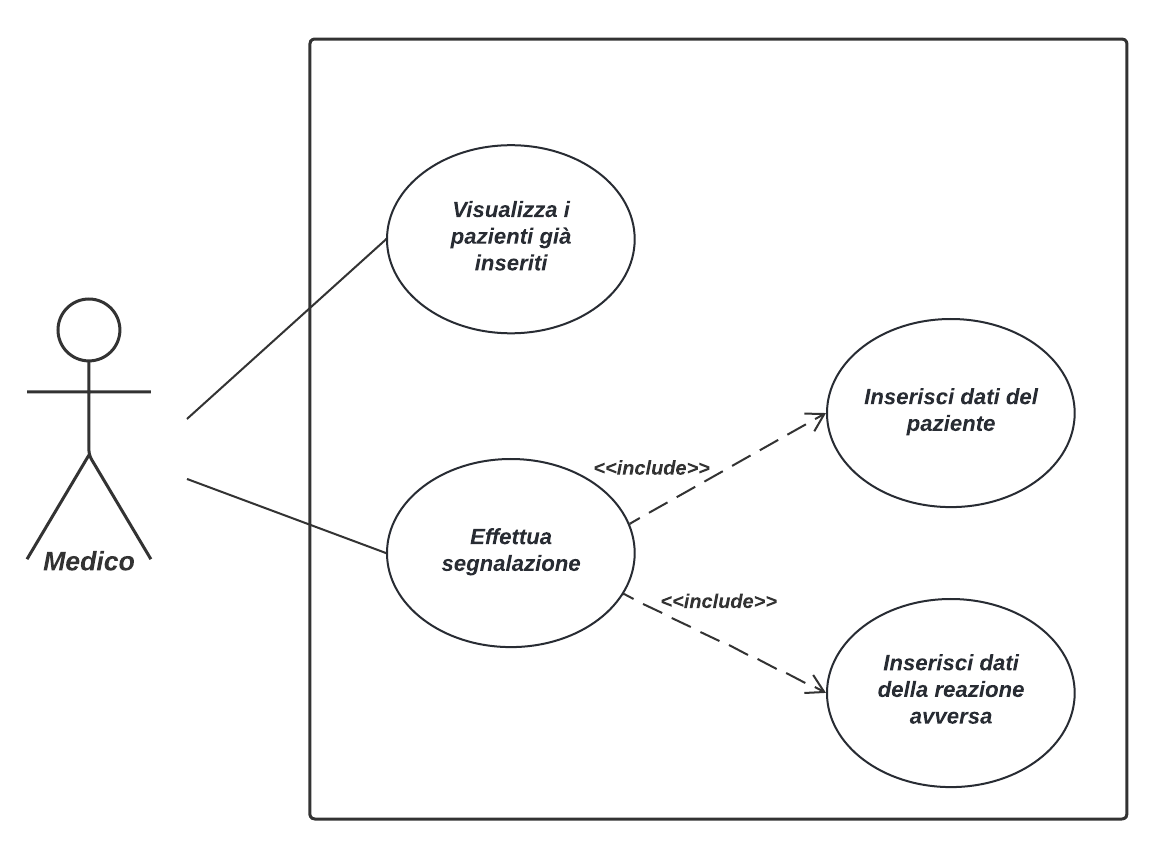
\includegraphics[width=0.75\textwidth]{pictures/CasoDUsoMedico.png}
            \captionof{figure}{Caso d'uso Medico}
            \end{center}
        Dopo opportuna autenticazione il medico viene introdotto all'interfaccia di base della sua sezione, che gli permette di:
            \begin{itemize}
                \item Visualizzare i pazienti già inseriti.
                \item Visualizzare i dati di un paziente dalla lista dei pazienti già inseriti.
                \item Effettuare una segnalazione.
            \end{itemize}
            \subparagraph*{Visualizza i pazienti}
            Una delle possibili attività che il Medico è autorizzato a fare è visualizzare la lista dei codici dei pazienti che lui stesso ha già inserito (gestiti automaticamente dal sistema), effettuando una segnalazione.
                \begin{center}
                    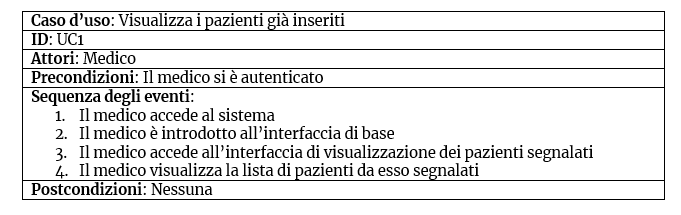
\includegraphics[width=0.75\textwidth]{pictures/UC1.png}
                \captionof{figure}{Caso d'uso UC1 del Medico}
            \end{center}

    \newpage
    Il medico può visualizzare anche le informazioni relative ai pazienti di cui vede i codici:
        \begin{center}
            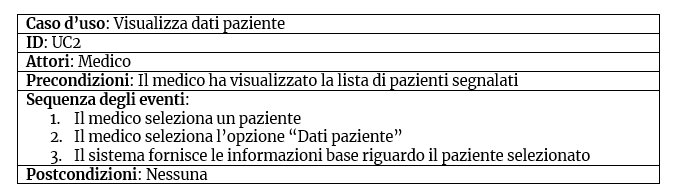
\includegraphics[width=0.75\textwidth]{pictures/UC2.png}
        \captionof{figure}{Caso d'uso UC2 del Medico}
        \end{center}
        Inseriamo ulteriori dettagli rispetto a questi due casi d'uso (gestiti in unico Sequence Diagram).
        \begin{center}
            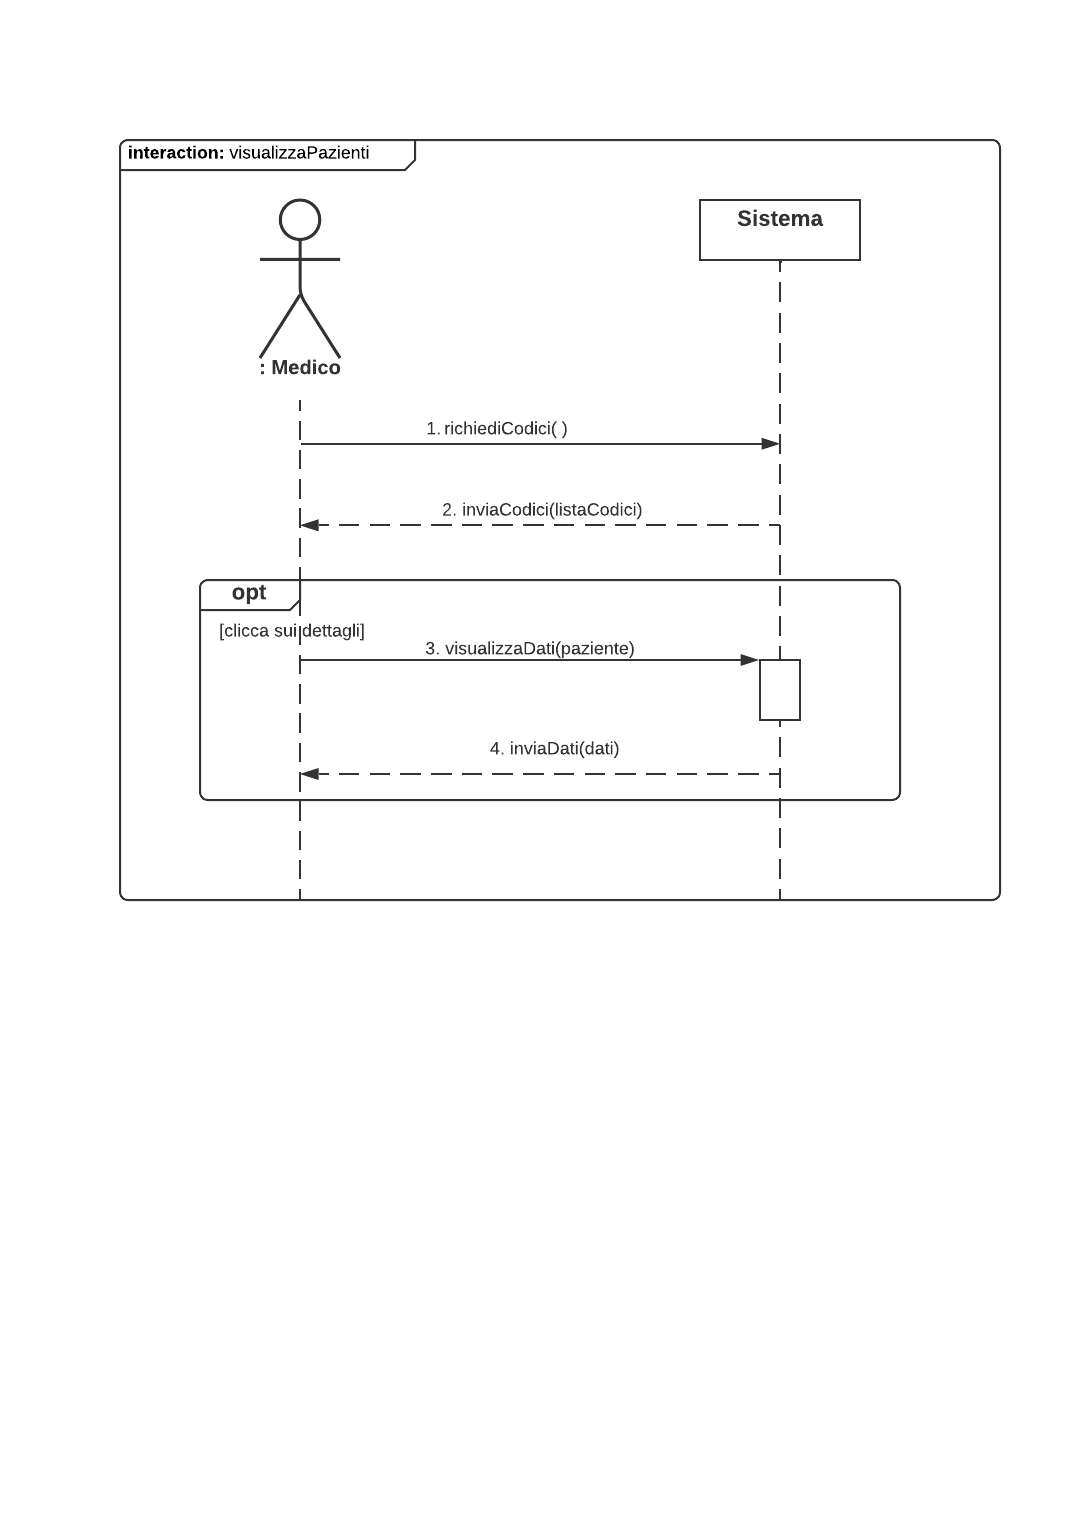
\includegraphics[width=0.80\textwidth]{pictures/SDMedico2_listaPazienti.png}
        \captionof{figure}{Sequence Diagram Visualizza Pazienti}
        \end{center}

    \newpage
        \subparagraph*{Effettua segnalazione}
            La principale attività dei medici è quella di inserire segnalazioni. Per fare questo, è necessario
            inserire i \textbf{dati del paziente} ed inserire i \textbf{dati della reazione avversa}. In questa sede si è scelto di non dare uno specifico ordine a queste due azioni: il medico potrà inserirle in ordine arbitrario.\\
            La data della segnalazione è gestita automaticamente dal sistema, al contrario della data della reazione avversa, che deve essere fornita esplicitamente.
                \begin{center}
                    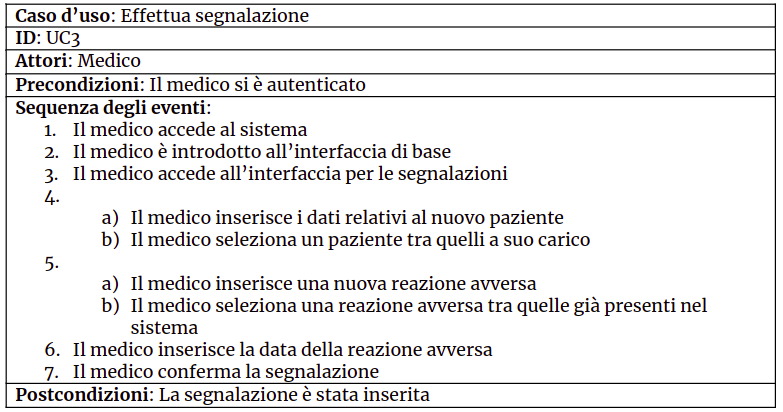
\includegraphics[width=0.65\textwidth]{pictures/UC3.png}
                \captionof{figure}{Caso d'uso UC3 del Medico}
                \end{center}
            In questa fase prevediamo l'inserimento dei dati, con diverse modalità.\\
            Per inserire i dati del paziente, abbiamo due alternative:
                \begin{itemize}
                    \item Inserire nuovi dati del paziente, effettuando quindi l'intera procedura di inserimento (dati anagrafici, fattori di rischio e storia vaccinale, in una sezione a parte)
                    \item Scegliere uno dei pazienti già inseriti nel sistema, in questo caso è possibile inserire nuove vaccinazioni ma l'azione non è obbligatoria.
                \end{itemize}
            L'identificativo univoco del paziente sarà gestito autonomamente dal sistema.\\
            Anche per l'inserimento dei dati della reazione avversa prevediamo due alternative:
                \begin{itemize}
                    \item Inserimento in sistema di una nuova reazione avversa, immettendo nome (univoco), gravità e descrizione.
                    \item Selezione di una reazione avversa nota, pre-esistente nel sistema.
                \end{itemize}
            Data la storia vaccinale del paziente e la data della segnalazione, il sistema gestisce autonomamente
            le vaccinazioni del paziente entro i due mesi precedenti la segnalazione.

    \newpage
    In ambo i casi, sarà necessario inserire la data della reazione avversa: questa dovrà essere consistente con la data della segnalazione.
        \begin{center}
            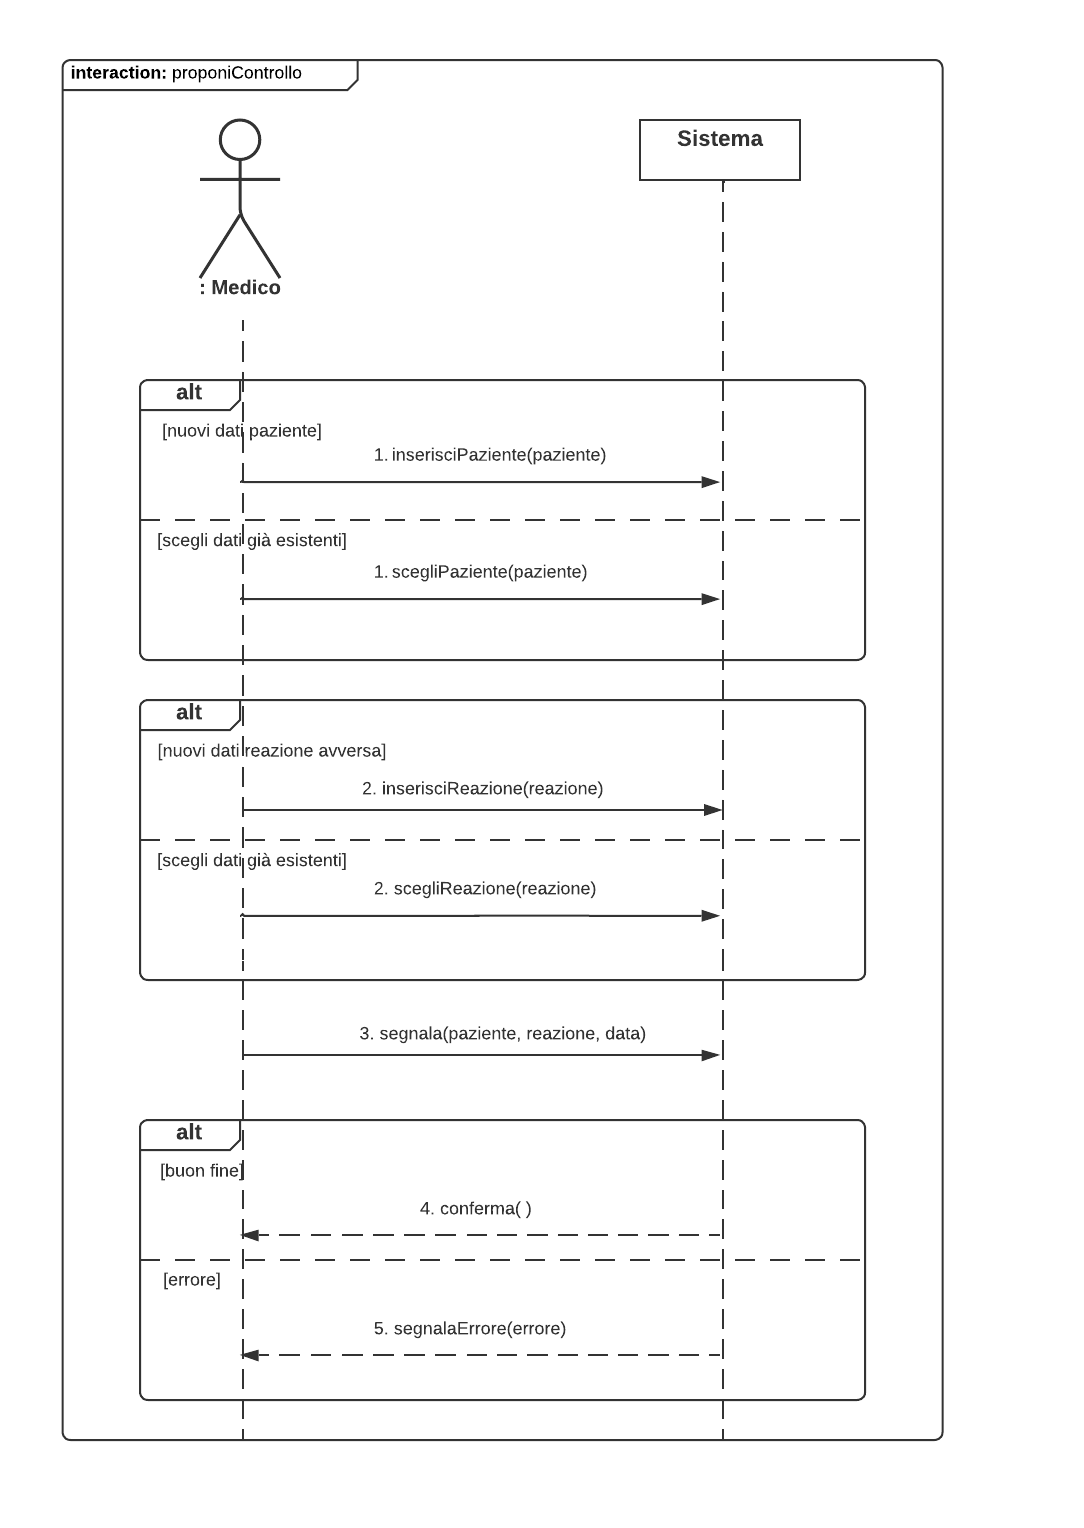
\includegraphics[width=0.80\textwidth]{pictures/SDMedico1_Segnalazione.png}
        \captionof{figure}{Sequence Diagram Effettua Segnalazione}
        \end{center}

    \newpage
        \paragraph*{Casi d'uso relativi al Farmacologo}
                \begin{center}
                    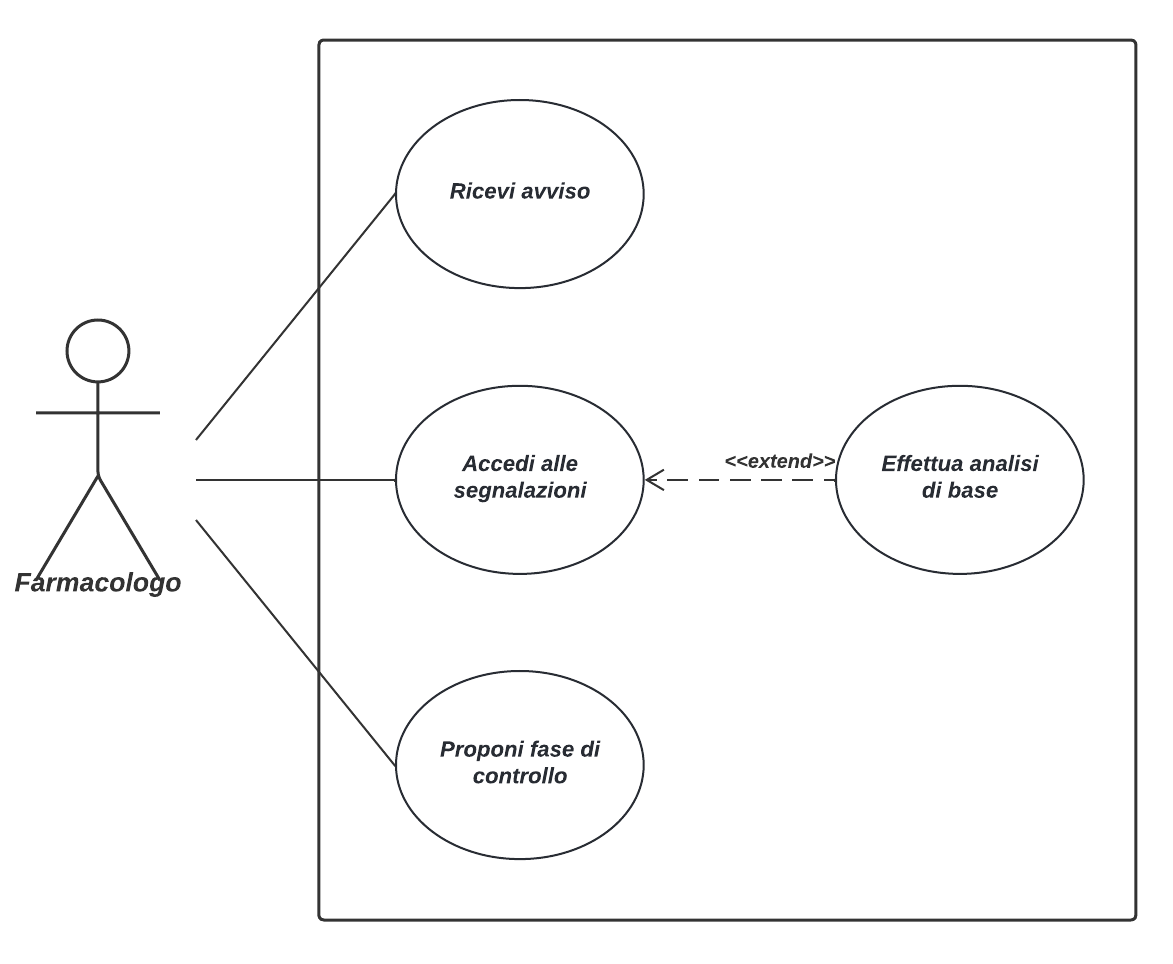
\includegraphics[width=0.75\textwidth]{pictures/CasoDUsoFarmacologo.png}
                \captionof{figure}{Caso d'uso Farmacologo}
                \end{center}
            Dopo opportuna autenticazione il farmacologo viene introdotto all'interfaccia di base della sua sezione. Prima di poter effettuare qualsiasi azione gli vengono mostrati gli \textbf{avvisi non letti}. Successivamente egli può:
                \begin{itemize}
                    \item Accedere alle segnalazioni
                    \item Dalle segnalazioni può effettuare delle analisi di base
                    \item Proporre delle fasi di controllo
                    \item Visualizzare gli avvisi già letti
                \end{itemize}
            \subparagraph*{Avvisi}
                Il sistema deve fornire un meccanismo di gestione ed invio di avvisi verso i
                farmacologi. Gli avvisi si dividono in tre tipologie:
                    \begin{enumerate}
                        \item Il sistema manda un avviso non specifico se sono state raggiunte le 50 segnalazioni in una settimana.
                        \item Il sistema manda un avviso non specifico se è il weekend.
                        \item Il sistema manda un avviso specifico rispetto ai vaccini, se questi hanno accumulato oltre 5 segnalazioni di gravità superiore a 3.
                    \end{enumerate}
                In questa sede si è deciso, nella casualità che durante il weeekend fossero state raggiunte le 50 segnalazioni in una settimana, di dare priorità a questo secondo avviso, non inviando un ulteriore avviso per il weekend.
            \newpage
                Il sistema avverte \textbf{tutti} i farmacologi responsabili. Ciò significa che ogni farmacologo all'autenticarsi riceverà gli avvisi generati e non ancora letti \textit{da lui}:
                questo avviene in forma di pop-up e prima di vedere la schermata iniziale.\\
                È inoltre possibile, tramite un'opzione nel menù principale, rivedere gli avvisi già letti.
                    \begin{center}
                        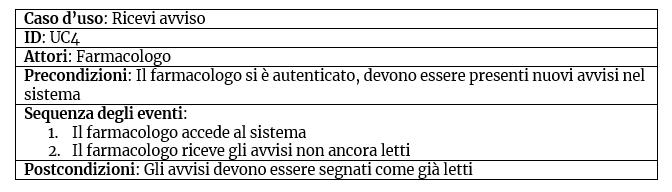
\includegraphics[width=0.75\textwidth]{pictures/UC4.png}
                    \captionof{figure}{Caso d'uso UC4 del Farmacologo}
                    \end{center}
                In fase di descrizione dei casi d'uso si è ritenuto opportuno inserire anche la possibilità di vedere gli avvisi già letti:
                    \begin{center}
                        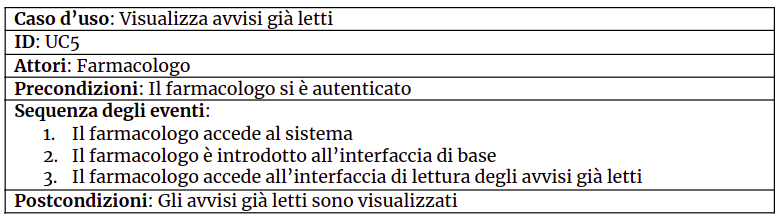
\includegraphics[width=0.75\textwidth]{pictures/UC5.png}
                    \captionof{figure}{Caso d'uso UC5 del Farmacologo}
                    \end{center}
            \subparagraph*{Leggi Segnalazioni}
                Il farmacologo può accedere alla lista delle segnalazioni:
                    \begin{center}
                        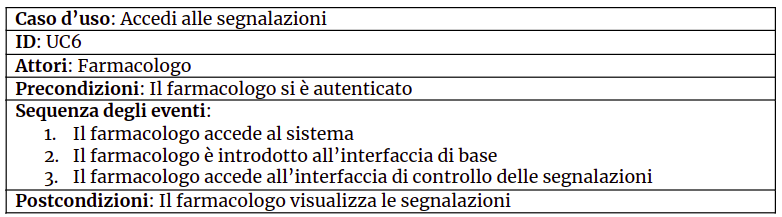
\includegraphics[width=0.75\textwidth]{pictures/UC6.png}
                    \captionof{figure}{Caso d'uso UC6 del Farmacologo}
                    \end{center}
                Nell'interfaccia dedicata alla lista delle segnalazioni vengono inseriti anche i dettagli relativi ad esse (codice del report, codice del dottore, nome della reazione, data del report e data della reazione, vaccinazioni del paziente relative ai due mesi precedenti alla reazione).

    \newpage
        \subparagraph*{Effettua analisi di base}
        Dalla lista delle segnalazioni il farmacologo può scegliere di effettuare delle \textbf{analisi di base}. Queste sono:
            \begin{itemize}
                \item Quante segnalazioni per vaccino, totali e negli ultimi sei mesi
                \item Quante segnalazioni gravi in settimana per vaccino
                \item Quante segnalazioni per provincia di residenza del paziente
                \item Quante segnalazioni per sede di vaccinazione
            \end{itemize}
            \begin{center}
                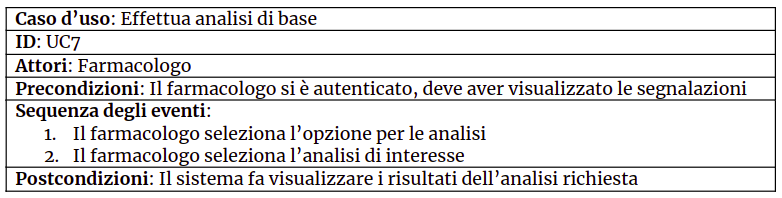
\includegraphics[width=0.75\textwidth]{pictures/UC7.png}
            \captionof{figure}{Caso d'uso UC7 del Farmacologo}
            \end{center}
        \subparagraph*{Propone Fase di Controllo}
            In base alle analisi eseguite e alla lettura delle segnalazioni, il farmacologo può proporre di attivare una fase di controllo del vaccino.\\
            Tale proposta viene registrata dal sistema.
                \begin{center}
                    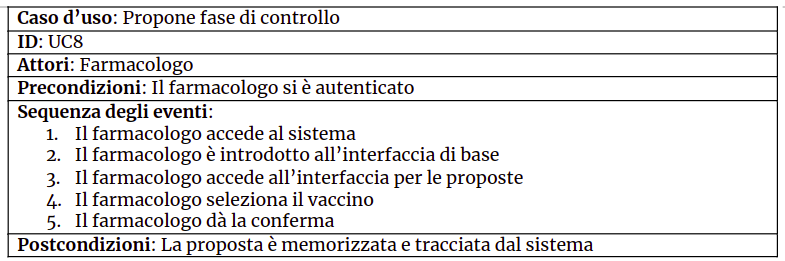
\includegraphics[width=0.75\textwidth]{pictures/UC8.png}
                \captionof{figure}{Caso d'uso UC8 del Farmacologo}
                \end{center}
            Si è deciso di non permettere ad un farmacologo di proporre due fasi di controllo per lo stesso vaccino nella stessa data.
                \begin{center}
                    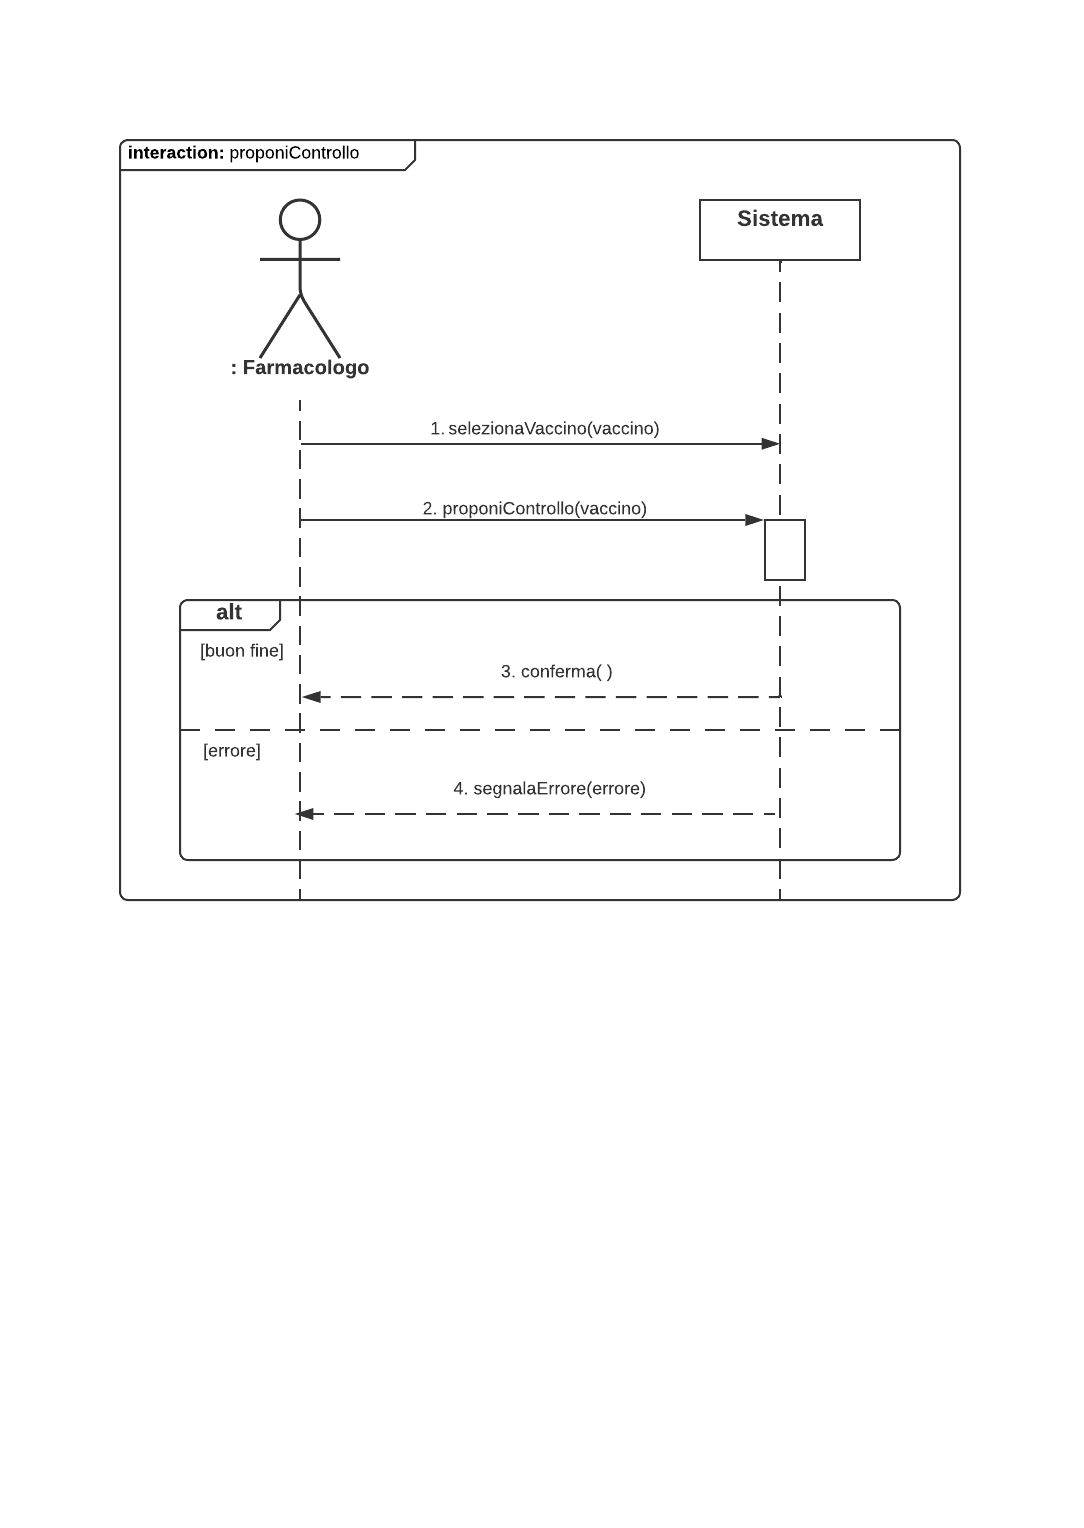
\includegraphics[width=0.80\textwidth]{pictures/SDFarmacolo2_proponeControllo.png}
                \captionof{figure}{Sequence Diagram 2 Farmacologo}
                \end{center}

    \newpage
        \subsection{Diagrammi di Attività}
            \subparagraph*{Nota sui diagrammi}
            Nei diagrammi relativi alle azioni successive al login non si è ritenuto di aggiungere una freccia che collega la scelta finale ad ogni interfaccia di partenza, per chiarezza e compattezza degli schemi.\\

            \paragraph*{Attività di Login}
                \begin{center}
                    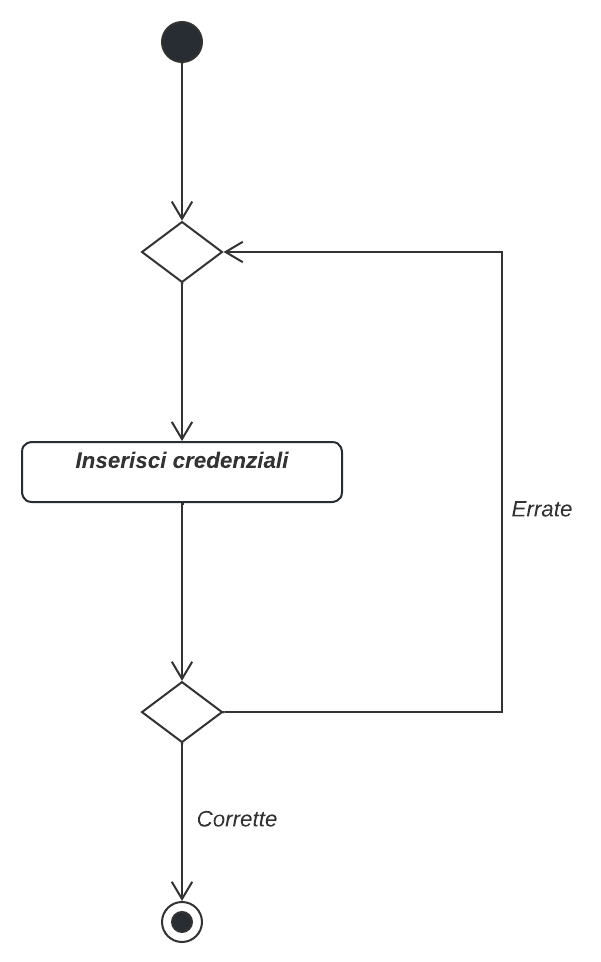
\includegraphics[width=0.60\textwidth]{pictures/ActivityDiagram_Login.png}
                \captionof{figure}{}
            \end{center}

    \newpage
        \paragraph*{Attività dell'attore medico}
            \begin{center}
                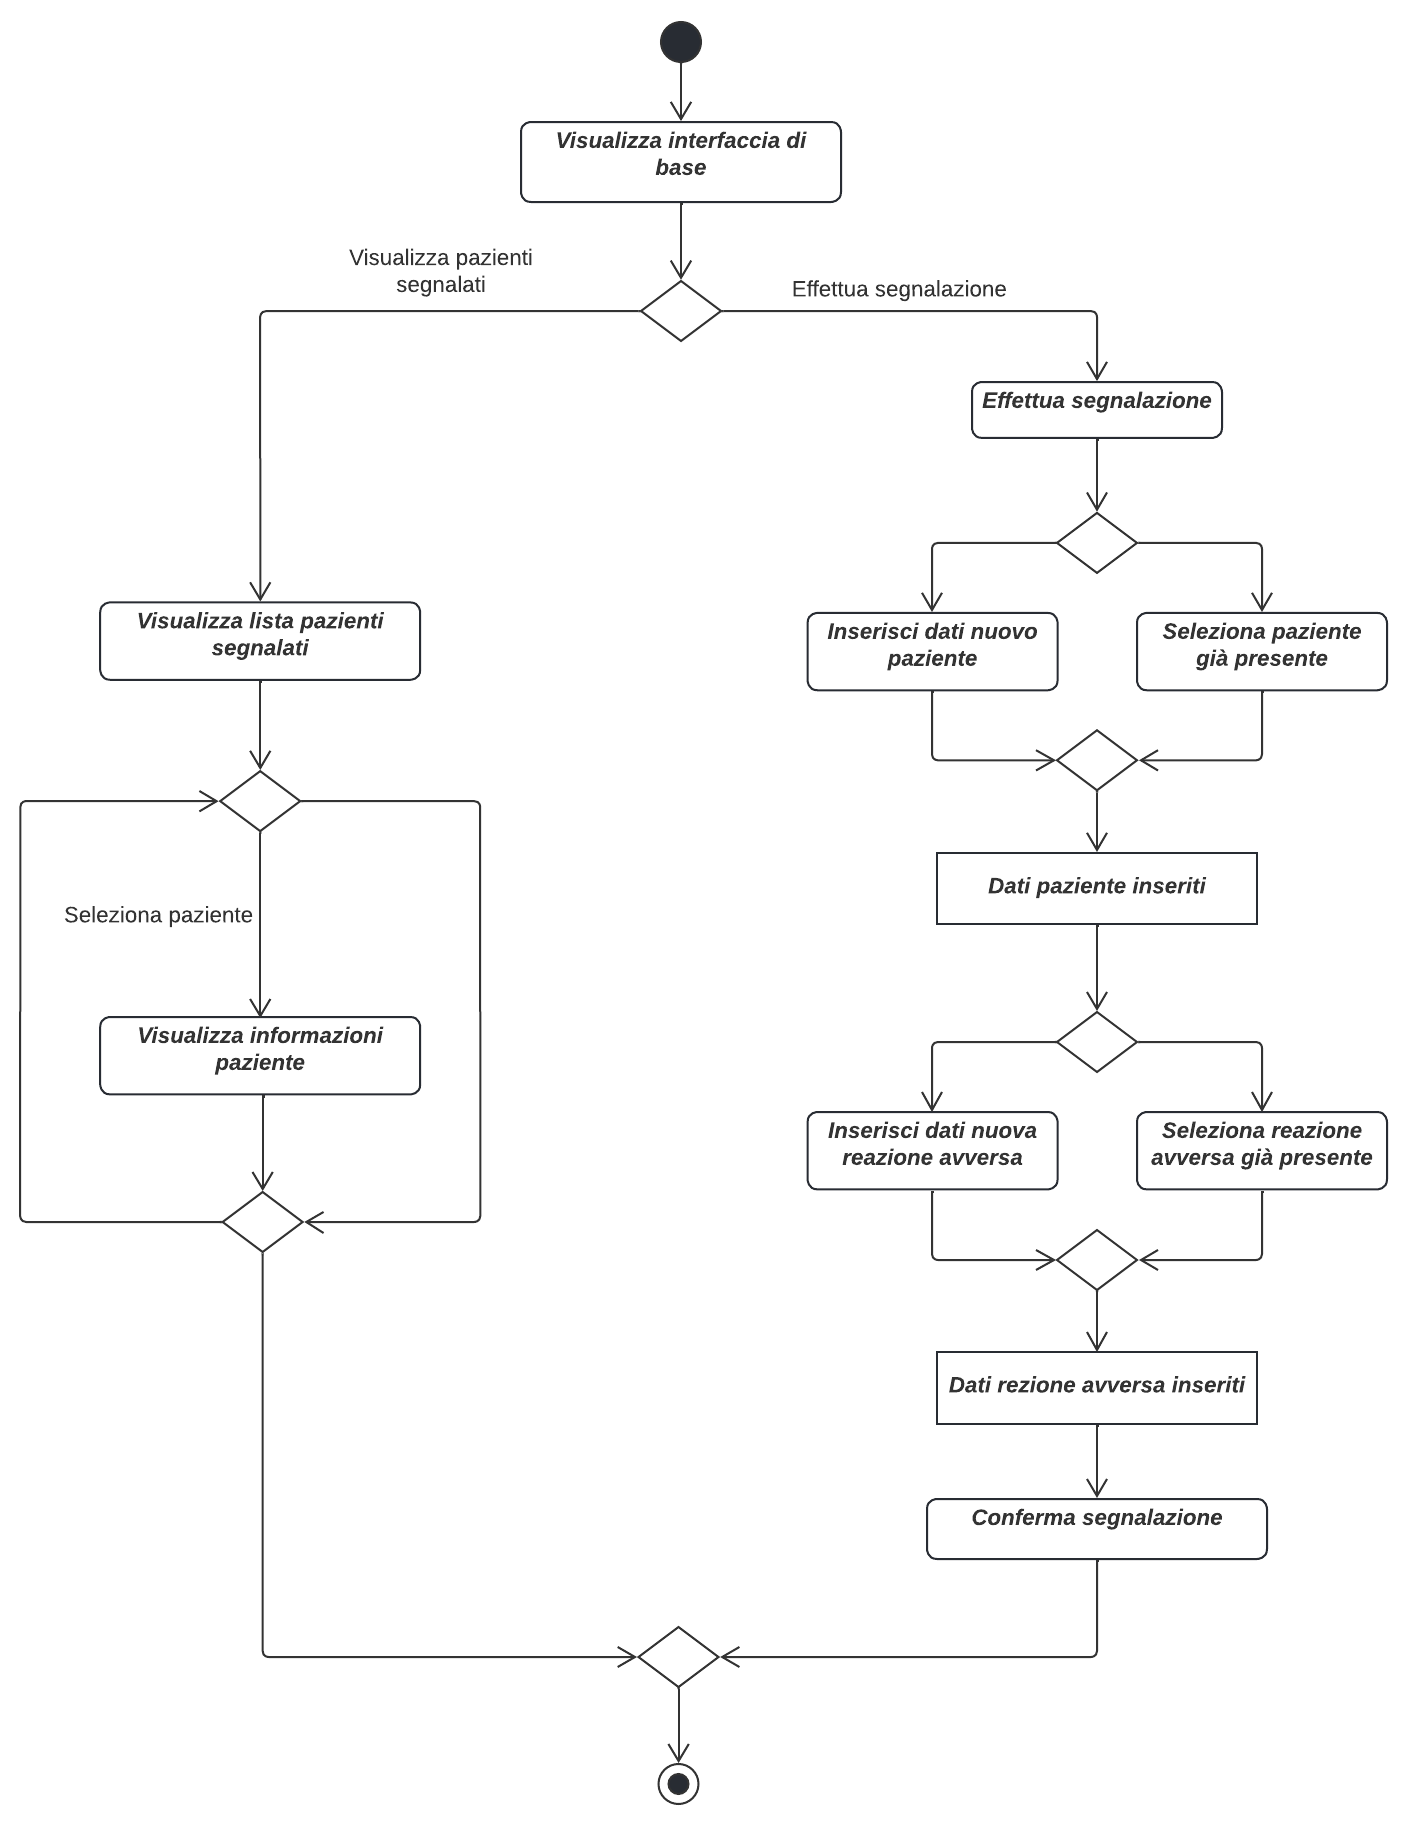
\includegraphics[width=1\textwidth]{pictures/ActivityDiagram_Medico.png}
            \captionof{figure}{}
            \end{center}

    \newpage
        \paragraph*{Attività dell'attore farmacologo}
            \begin{center}
                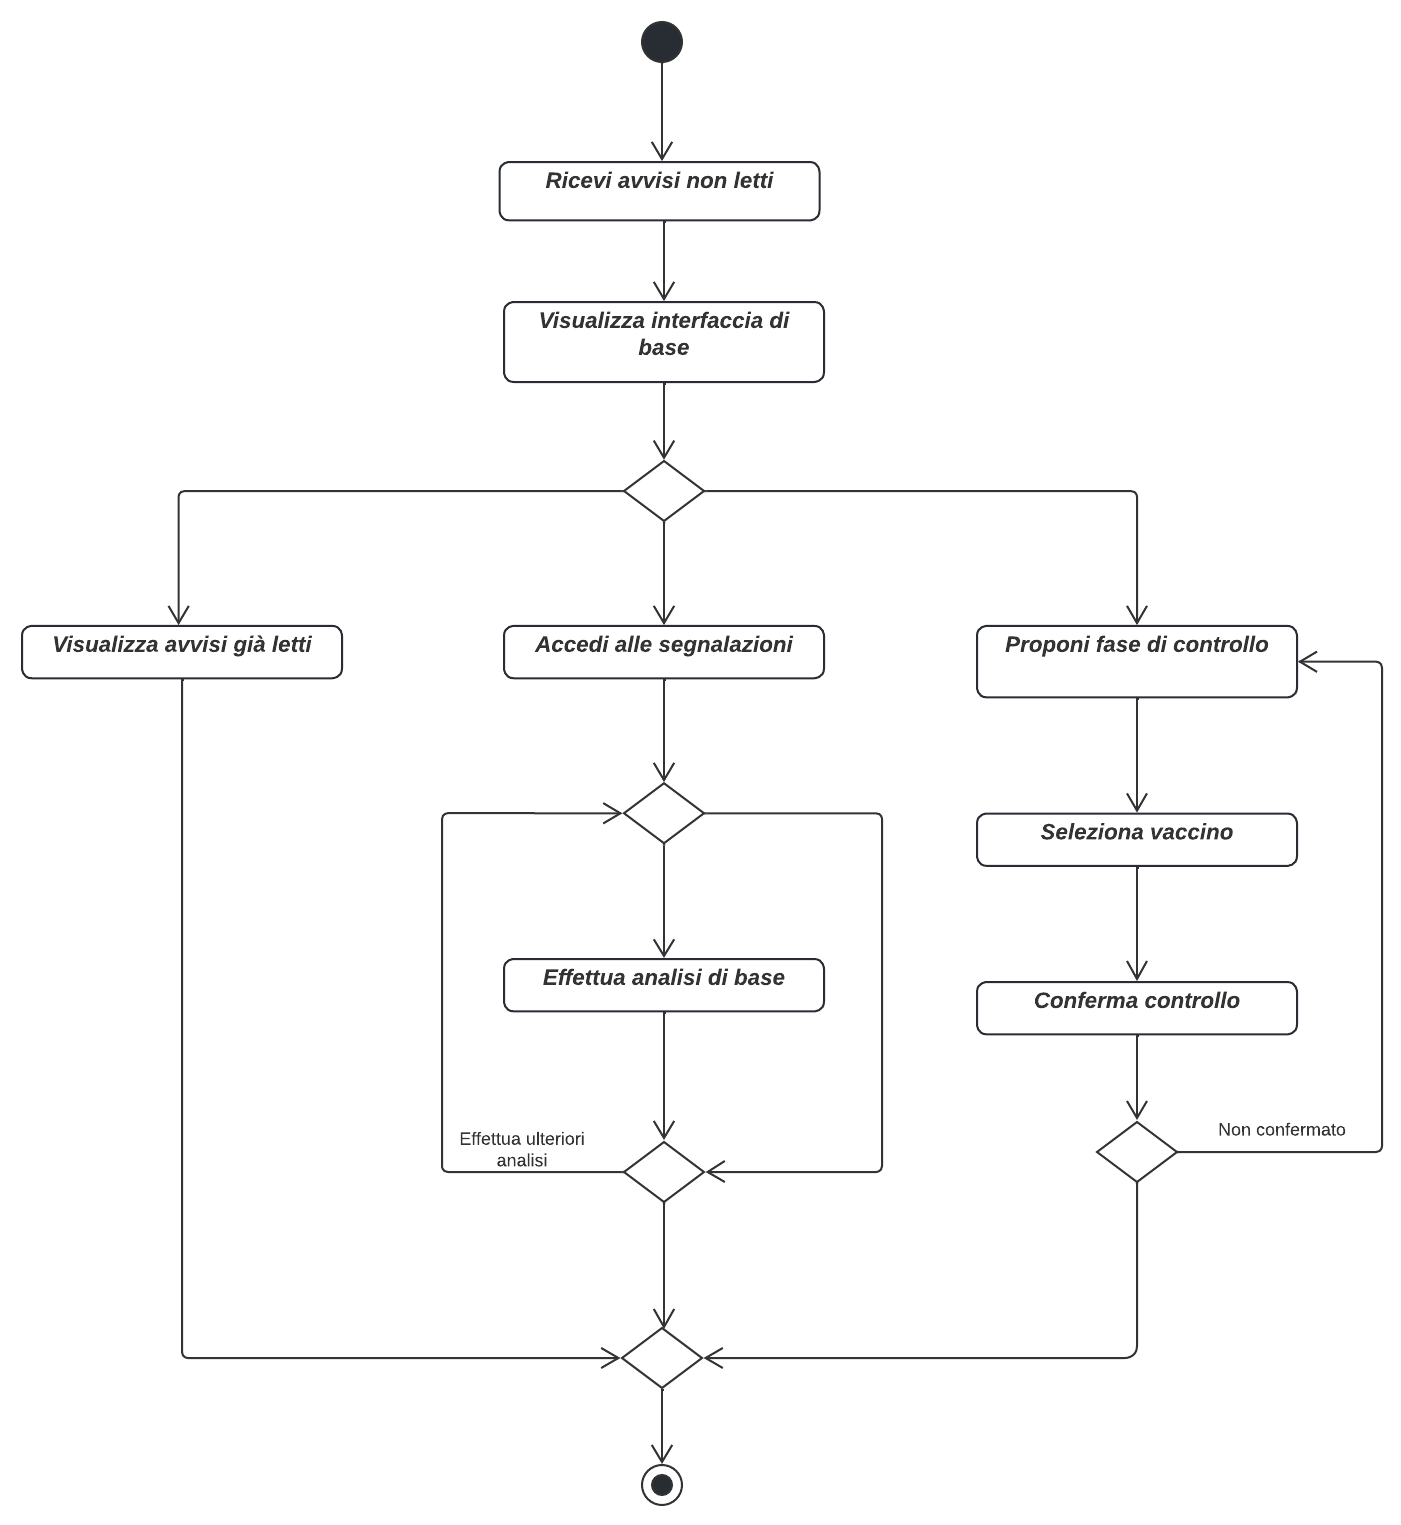
\includegraphics[width=1\textwidth]{pictures/ActivityDiagram_Farmacologo.png}
            \captionof{figure}{}
            \end{center}

    \newpage
    \section{Scelte progettuali}
        \subsection{Note sullo sviluppo}
        Si è scelto di sviluppare l'applicazione in Java, utilizzando la libreria \textbf{JavaFX}, senza l'ausilio di FXML, perché soddisfatti del design delle interfacce.\\
        Il progetto è stato interamente sviluppato utilizzando \textbf{Git} come sistema di \textit{code versioning} e GitHub per l'hosting della repository.\\
        Abbiamo seguito una metodologia di sviluppo per lo più a cascata e \textbf{Plan Driven}: le fasi di specifica e di sviluppo sono state separate, cercando di porre comunque rimedio al principale svantaggio dello stesso, ovvero la difficoltà di cambiamento dopo aver avviato il processo. Questo è stato fatto utilizzando alcune metodologie proprie dello \textbf{sviluppo Agile}, soprattutto l'attività di \textit{Pair Programming} che ha riguardato tutto lo sviluppo, con particolare attenzione allo sviluppo dei Modelli e delle prime View (si veda in seguito).\\
        Ogni area è stata divisa in task in modo da alleggerire il carico di lavoro e i design pattern sono stati scelti nella fase di sviluppo in base a quelle che erano le nostre necessità, al fine di ottenere un codice performante ma allo stesso tempo leggibile.\\
        Prima di cominciare lo sviluppo vero e proprio, si è condotta la fase di analisi dei requisiti che si è vista nella sezione precedente, generando i relativi use-cases e i diagrammi di attività. Anche la progettazione architetturale è stata fatta prima di iniziare il lavoro centrale, in
        modo da non avere problemi su quel frangente.

        \subsection{Pattern Architetturale - MVC}
        Abbiamo deciso di utilizzare il \textbf{pattern Model View Controller}, semplicemente perchè naturalmente implementabile con l'uso di JavaFX. Il sistema è strutturato in tre componenti logiche che interagiscono tra loro.\\
        Il \textbf{model} si occupa della gestione dei dati e delle operazioni su di essi. La componente \textbf{View} definisce le interfacce e come i dati vengono presentati all'utente. Il \textbf{Controller} 
        gestisce infine l'interazione delle interfacce e dell'utente con i dati.
            \begin{center}
                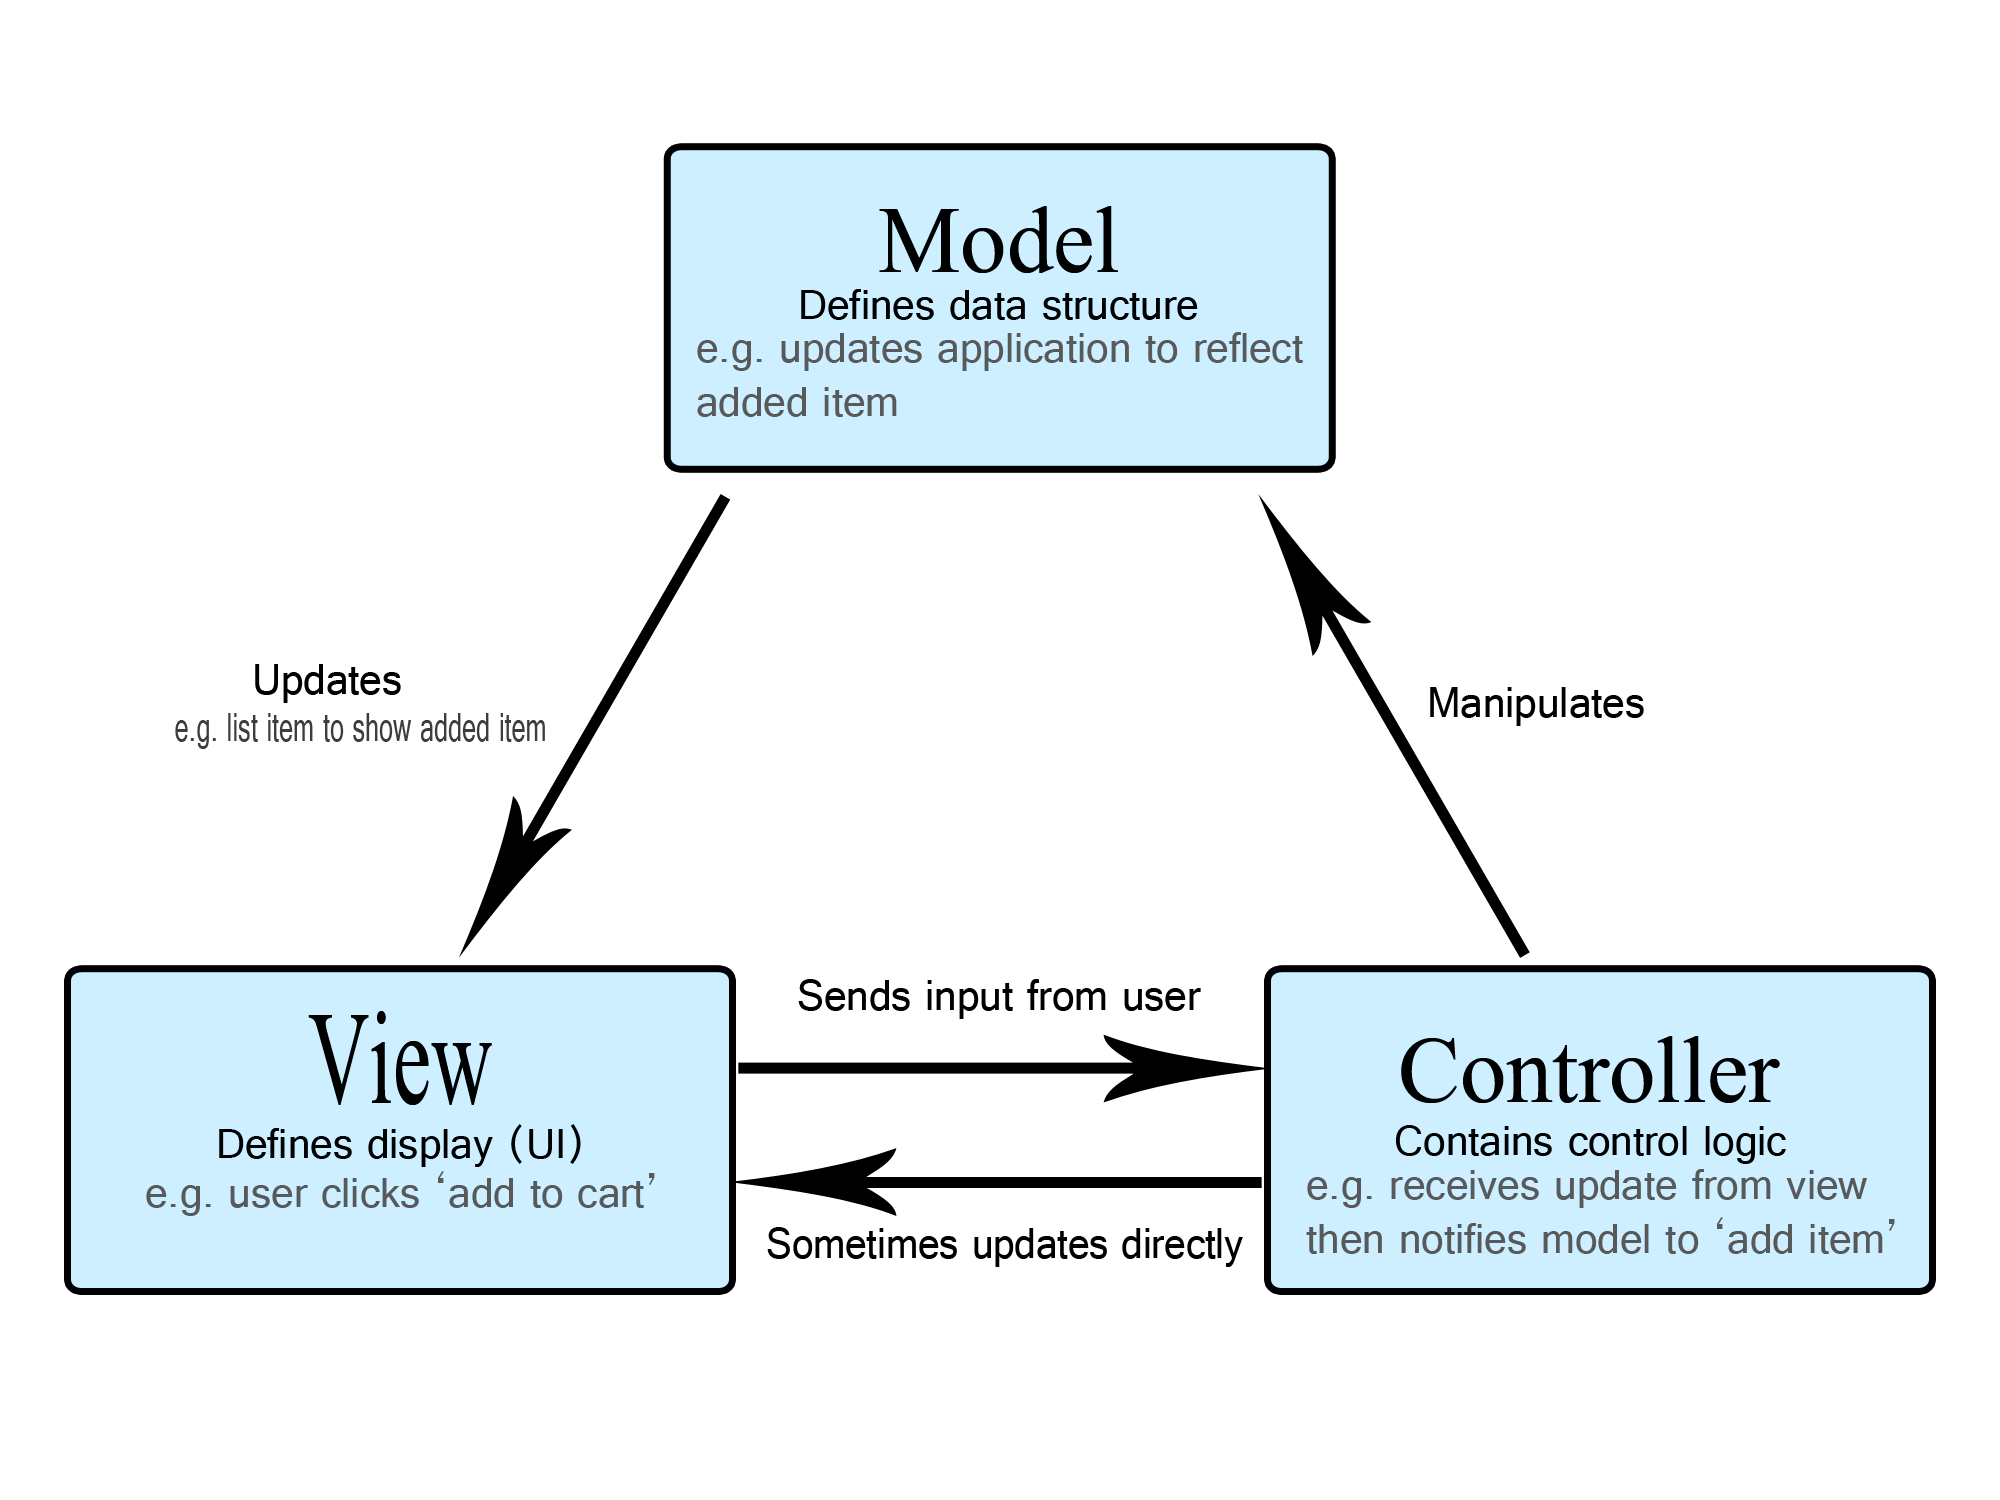
\includegraphics[width=0.70\textwidth]{pictures/mvc.png}
            \end{center}
            
    \newpage

        \subsection{Data Access Object Pattern}
            Per la gestione dei dati si è ritenuto di utilizzare il pattern DAO, utilizzato per separare i dati di basso livello che accedono all'API dalle operazioni di alto livello.\\
            Per ogni classe del Model (e di conseguenza per quasi tutte le tabelle implementate nel DataBase) si è implementato:
                \begin{itemize}
                    \item \textbf{Interfaccia DAO} - Definisce le operazioni standard da eseguire.
                    \item \textbf{Classe concreta DAO} - Implementa l'interfaccia di cui sopra. È responsabile dell'accesso ai dati dal database.
                    \item \textbf{Model Object} - Questo è un semplice oggetto Java che contiene i metodi getter e setter per memorizzare i dati.
                \end{itemize}
            Le classi-modello implementate con il pattern DAO sono (in ordine alfabetico):
                \begin{itemize}
                    \item \textbf{ControlPhase} - le fasi di controllo proposte dal farmacologo.
                    \item \textbf{Notice} - gli avvisi ricevuti dal farmacologo.
                    \item \textbf{Patient} - i pazienti.
                    \item \textbf{Reaction} - le reazioni avverse.
                    \item \textbf{Report} - le segnalazioni effettuate dai medici.
                    \item \textbf{RiskFactor} - i fattori di rischio relativi ai pazienti.
                    \item \textbf{Vaccination} - le vaccinazioni effettuate dai pazienti.
                \end{itemize}

            \paragraph*{Nota}
            Per la classe \textbf{User} (gli utenti che hanno accesso all'applicazione, ovvero dottori e farmacologi) si è deciso di non modellare la classe secondo il pattern DAO, ma di implementarla come un oggetto Java generico.

    \newpage
        \subsection{Diagrammi delle classi}
        \paragraph*{Classi del Modello}
            \begin{center}
                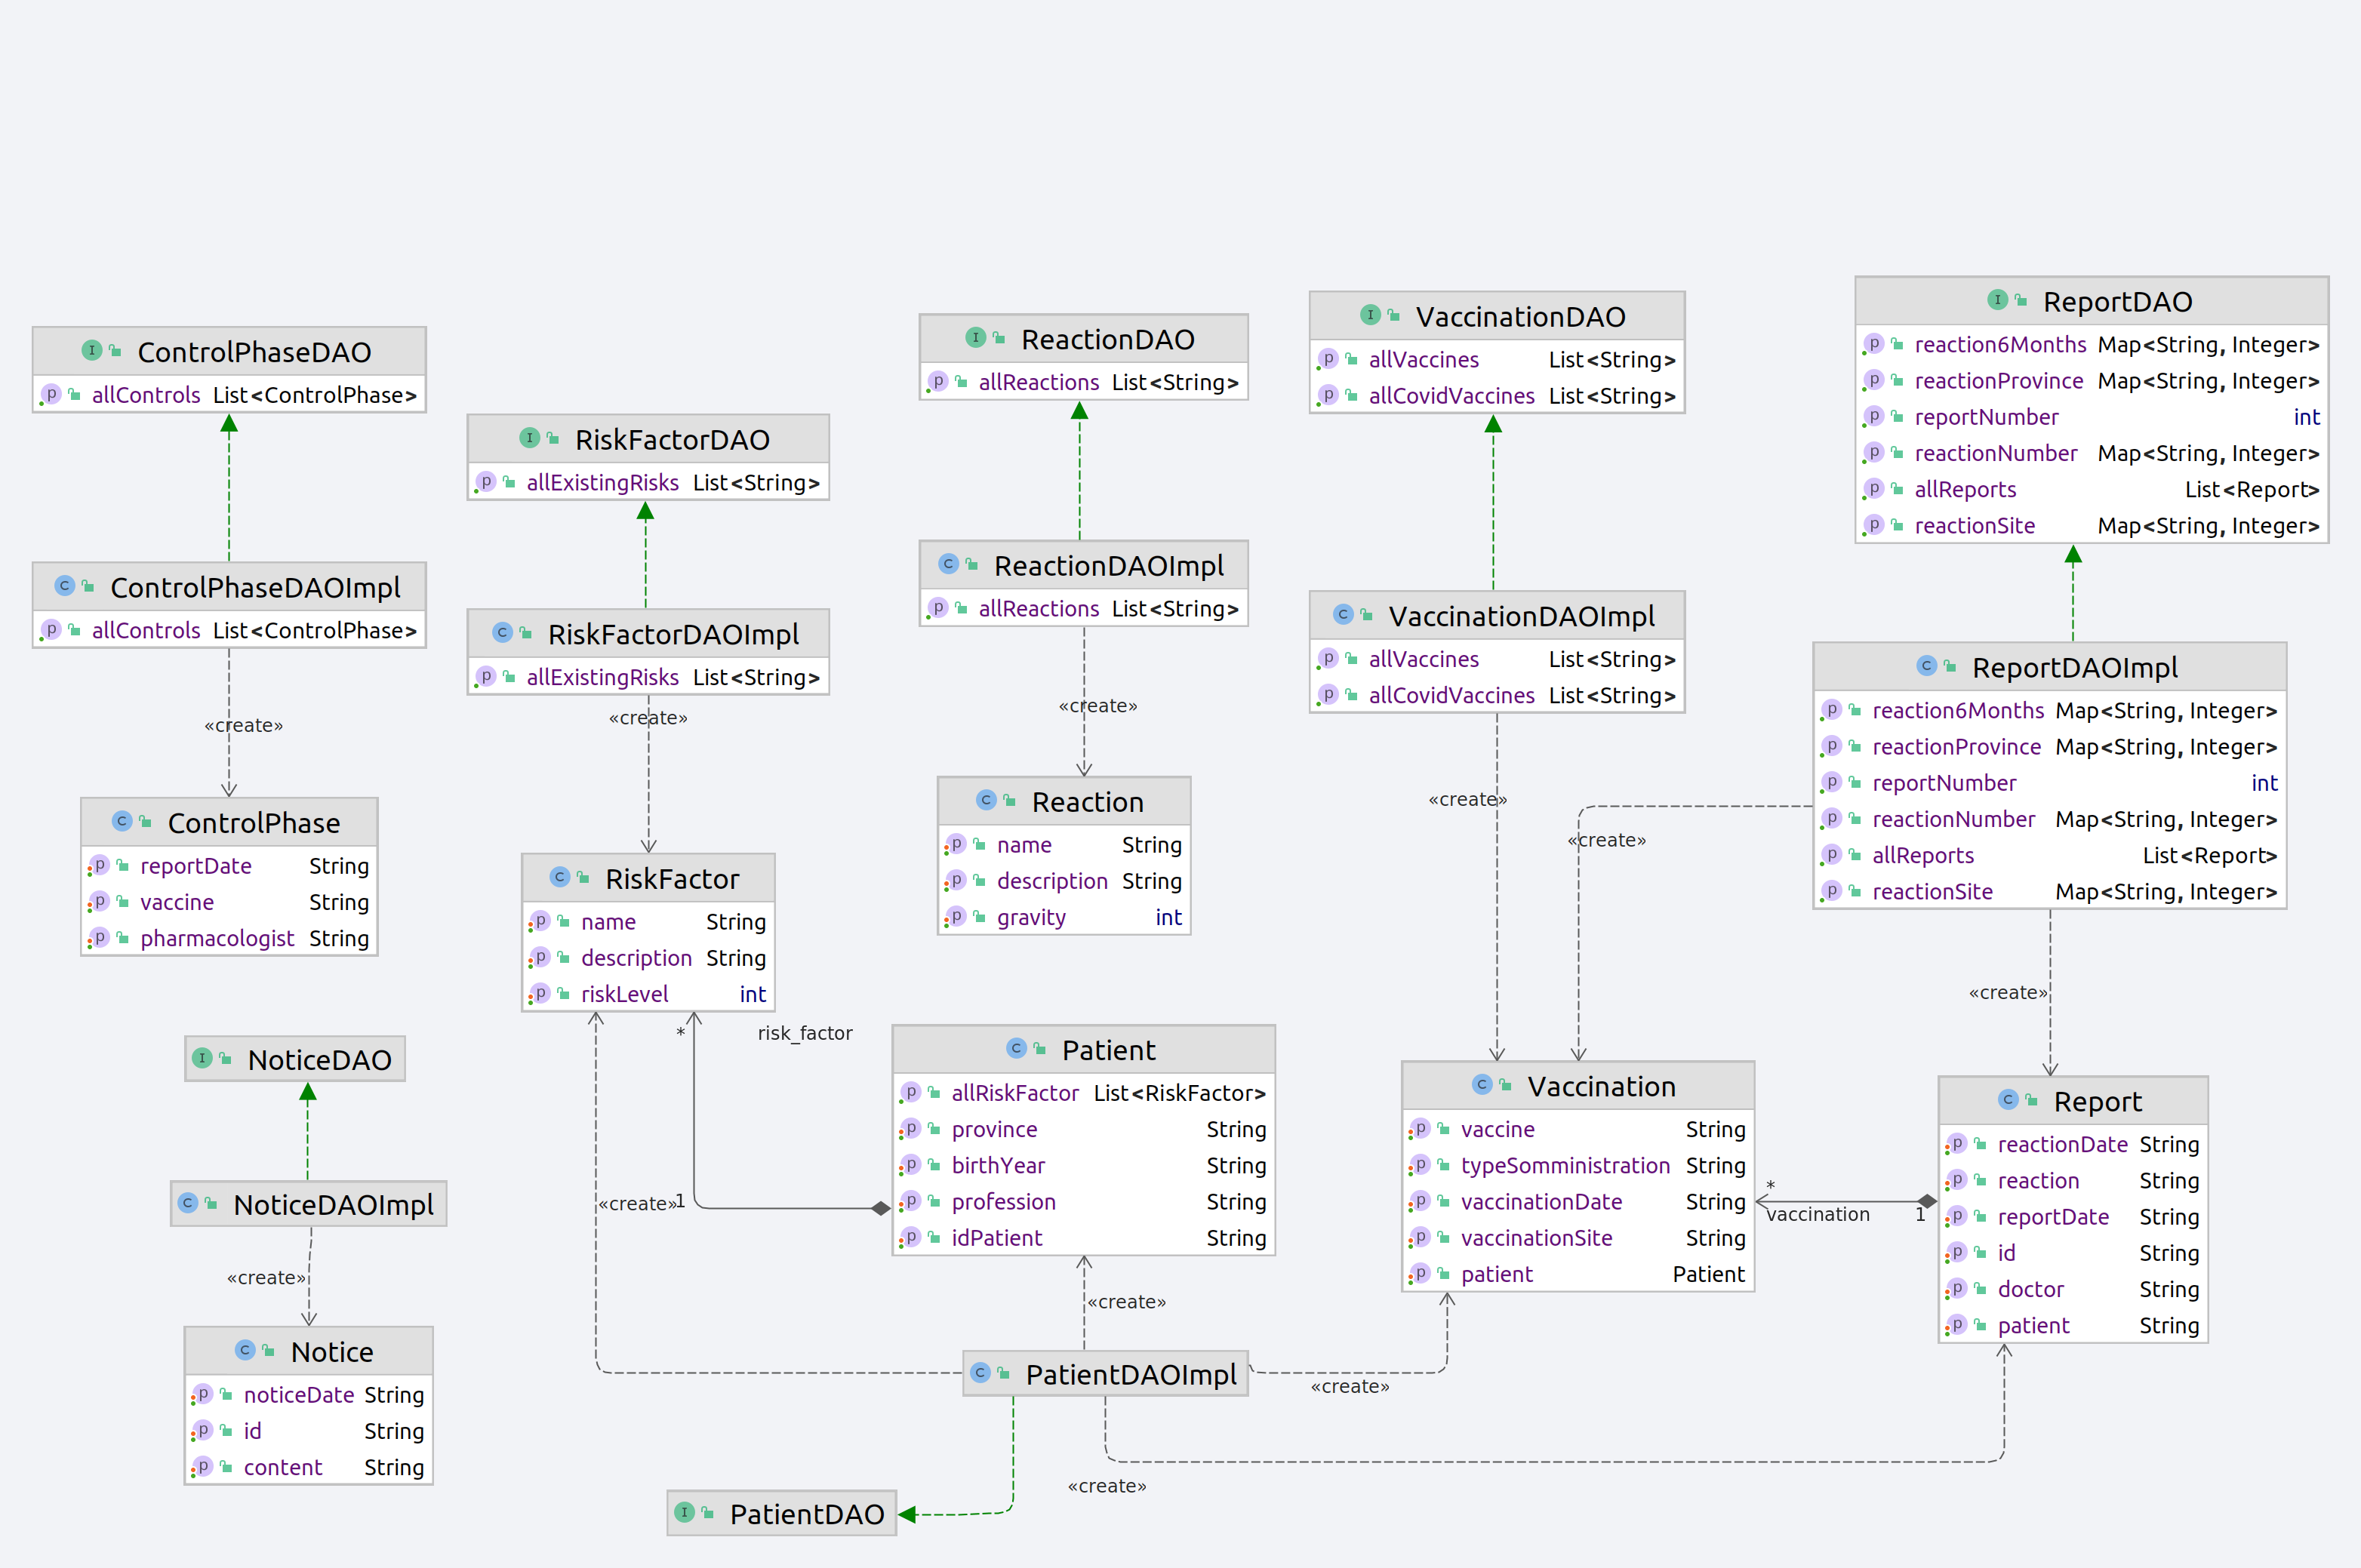
\includegraphics[width=1\textwidth]{pictures/DAOInteraction.png}
            \captionof{figure}{Interazione tra le classi del modello}
            \end{center}
        \newpage
            \paragraph*{Classi della View}
                \subparagraph*{Nota} Non si sono inserite nel diagramma le classi considerate \textit{Utils}, quindi le classi che ad esempio generano gli avvisi, i messaggi di errore o la lista dei vaccini possibili.
                \begin{center}
                    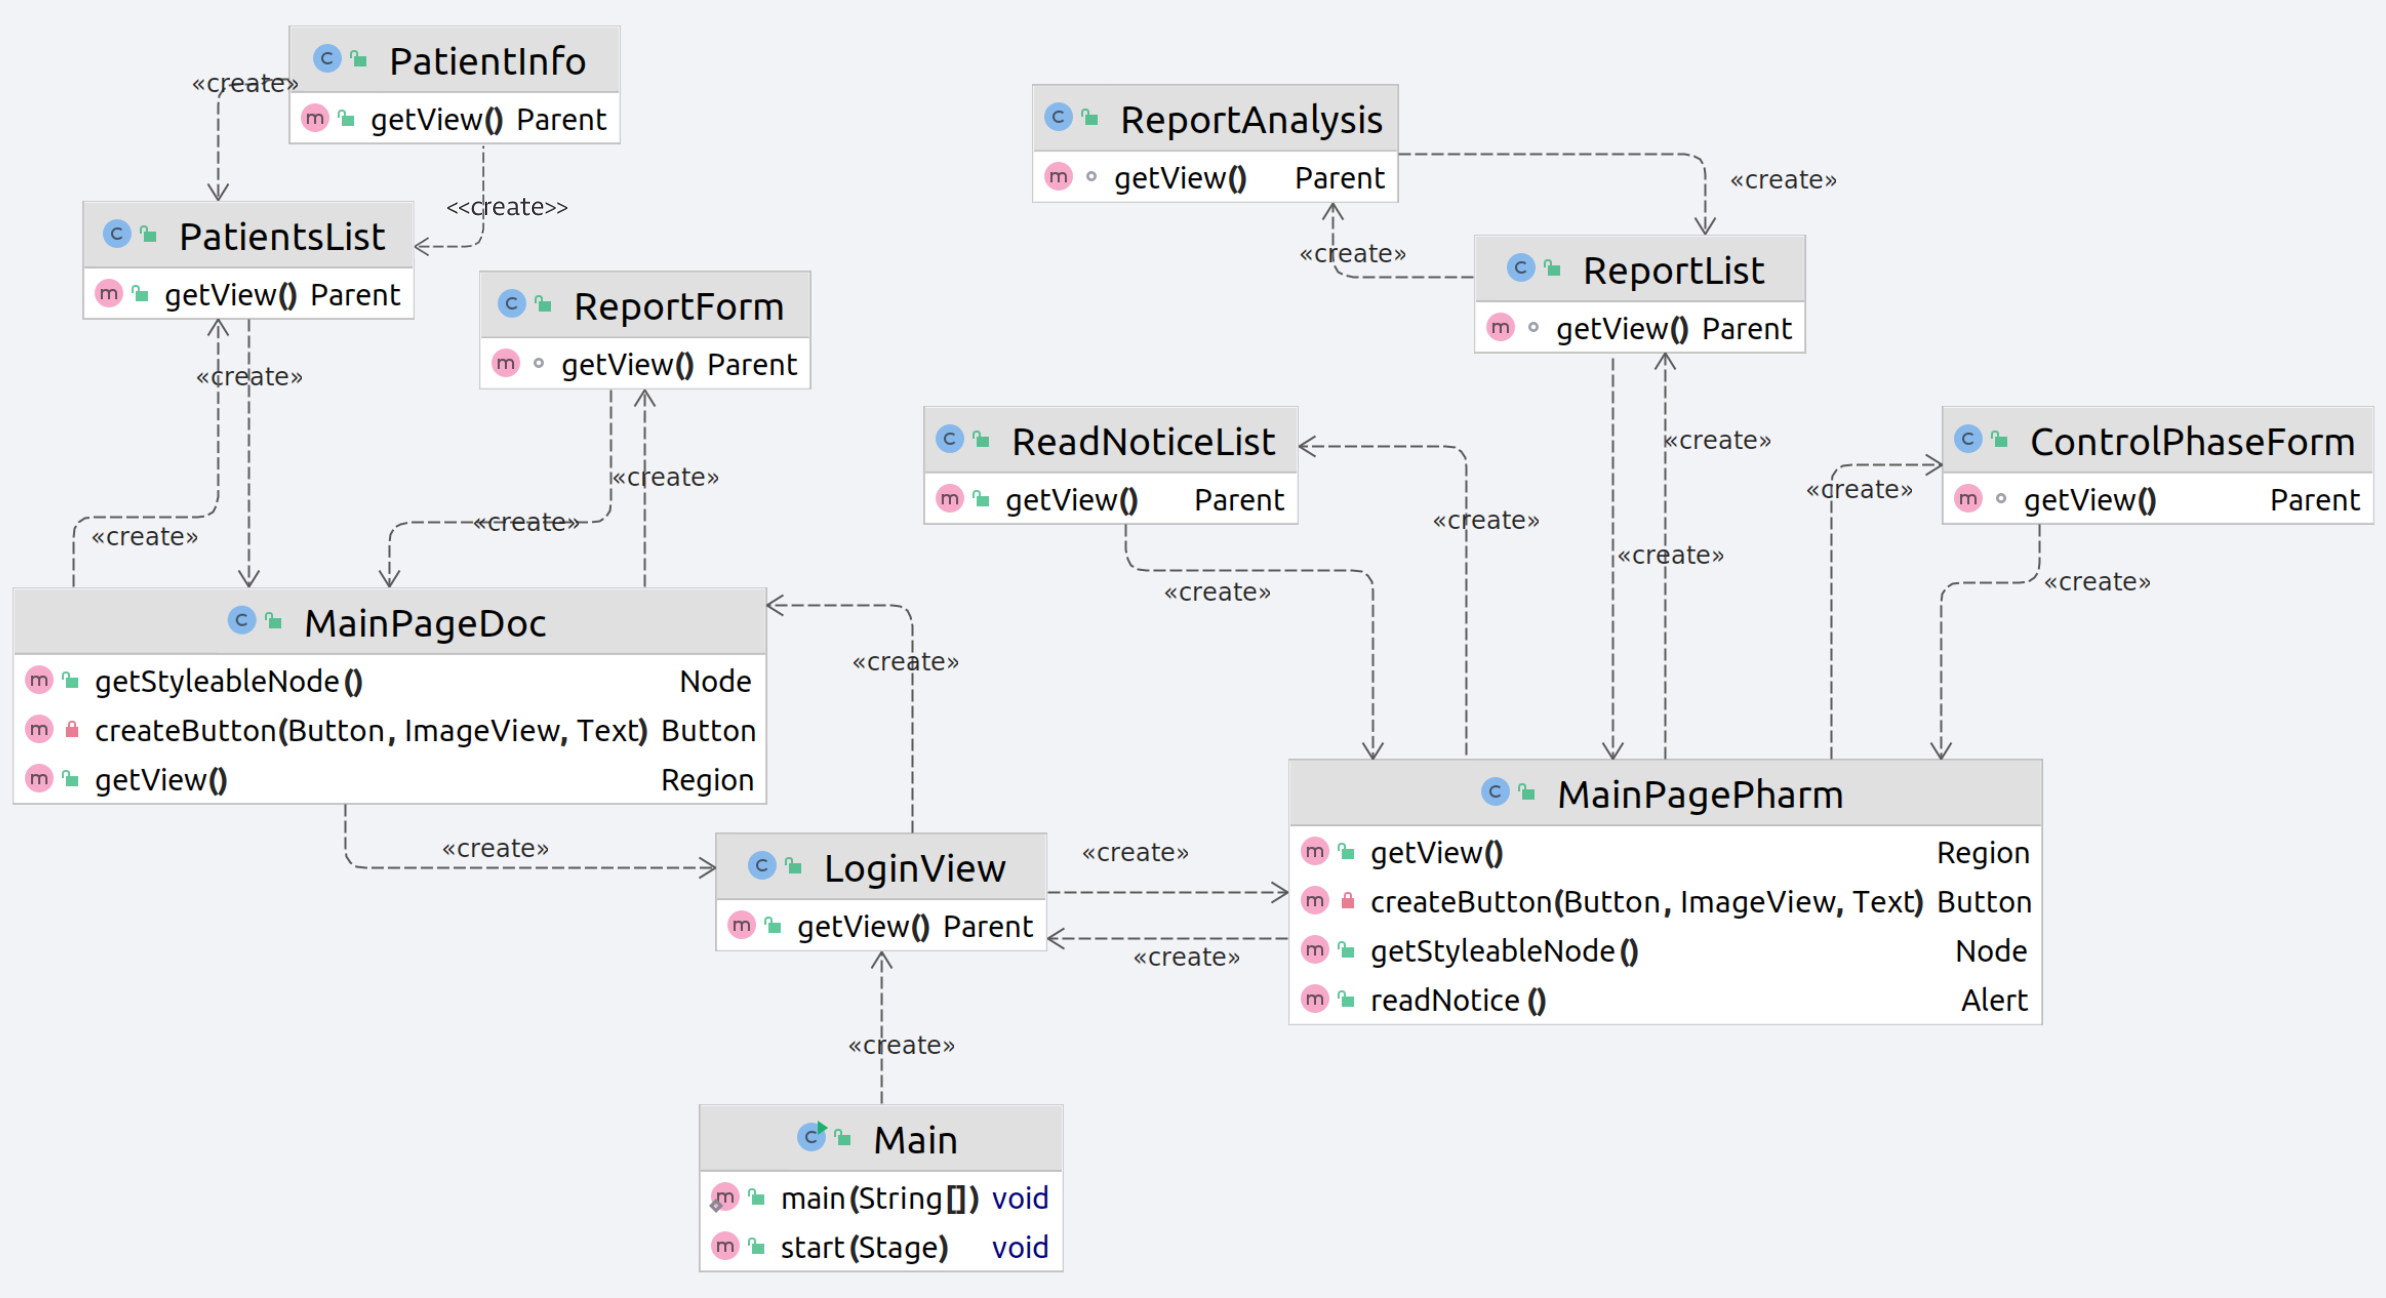
\includegraphics[width=1\textwidth]{pictures/ViewInteraction.png}
                \captionof{figure}{Interazione tra le classi della View}
                \end{center}
        \newpage
            \paragraph*{Esempio Interazione View - Controller}
                \subparagraph*{Nota} Si è scelto di riportare come \textit{Class Diagram} solo un esempio di \textbf{interazione tra Vista e Controllore}, perché esemplificativa delle interazioni generali tra questi due.\\
                La vista chiama i metodi del controllore per poter interagire con i dati, a cui il controllore ha accesso (si veda la prossima DAO).
                \begin{center}
                    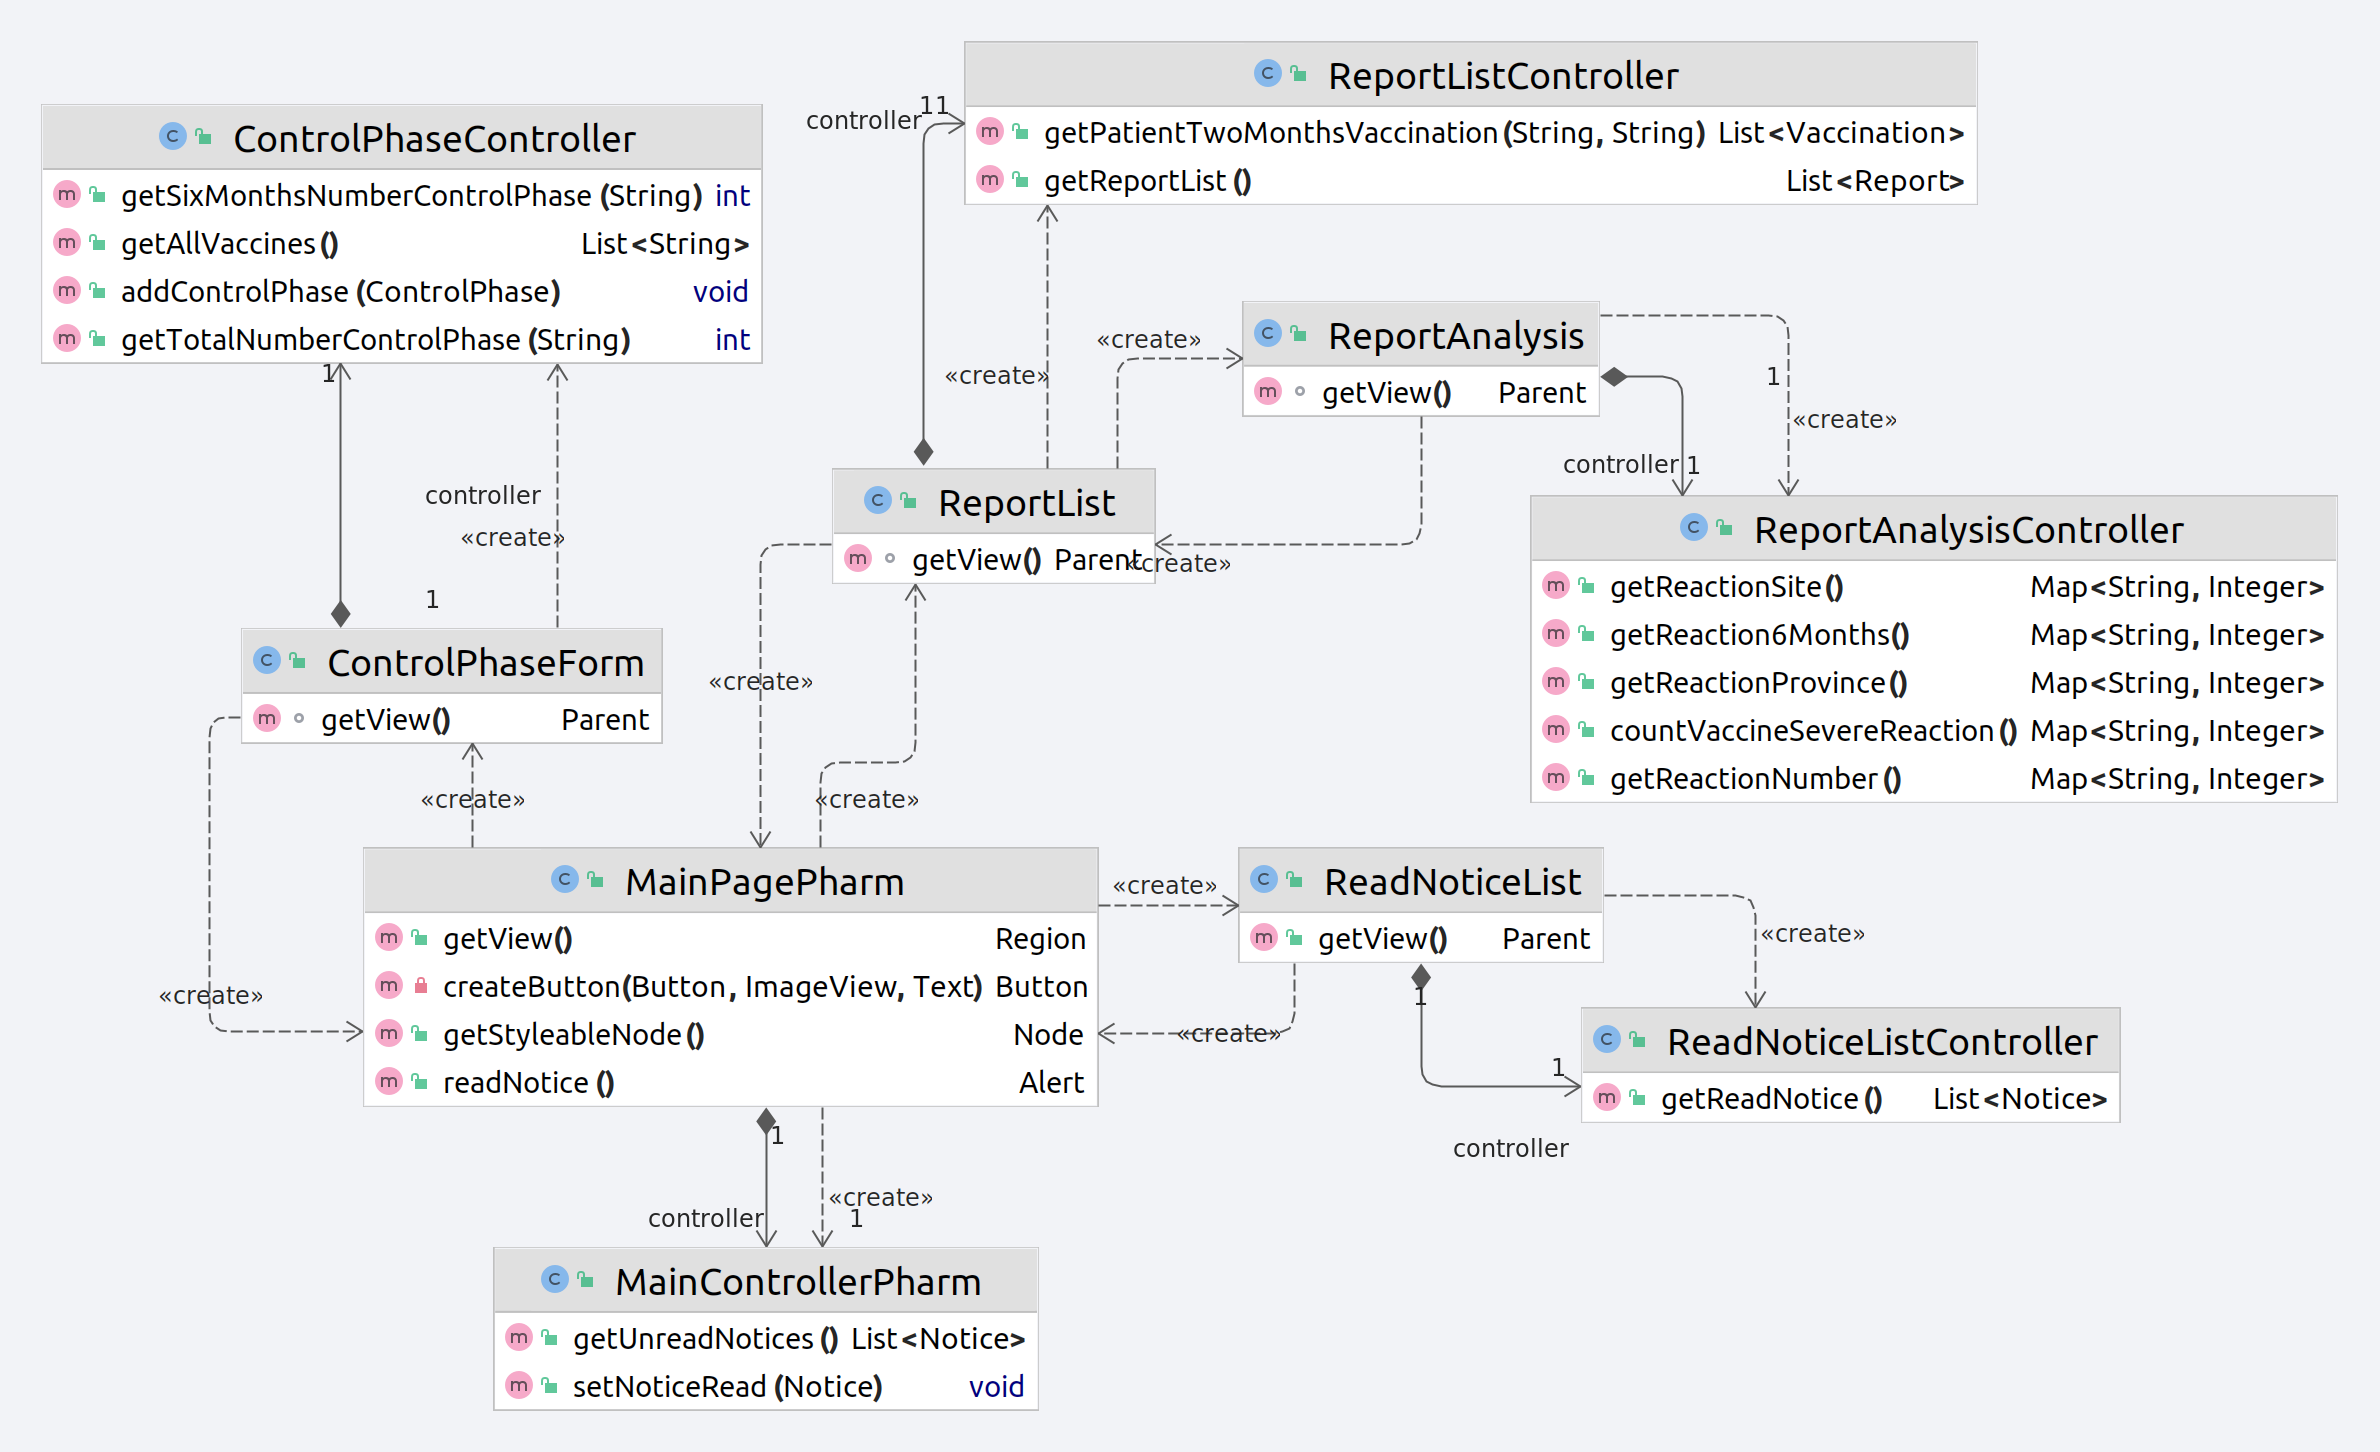
\includegraphics[width=1\textwidth]{pictures/ExampleControlViewInteraction.png}
                \captionof{figure}{Interazione tra le classi della View Farmacologo e i loro controller}
                \end{center}
        \newpage
            \paragraph*{Esempio Interazione DAO - Controller}
            \subparagraph*{Nota} Si è scelto anche in questo caso di riportare come \textit{Class Diagram} solo un esempio di \textbf{interazione tra Vista e Controllore}, perché esemplificativa delle interazioni generali tra questi due.
                \begin{center}
                    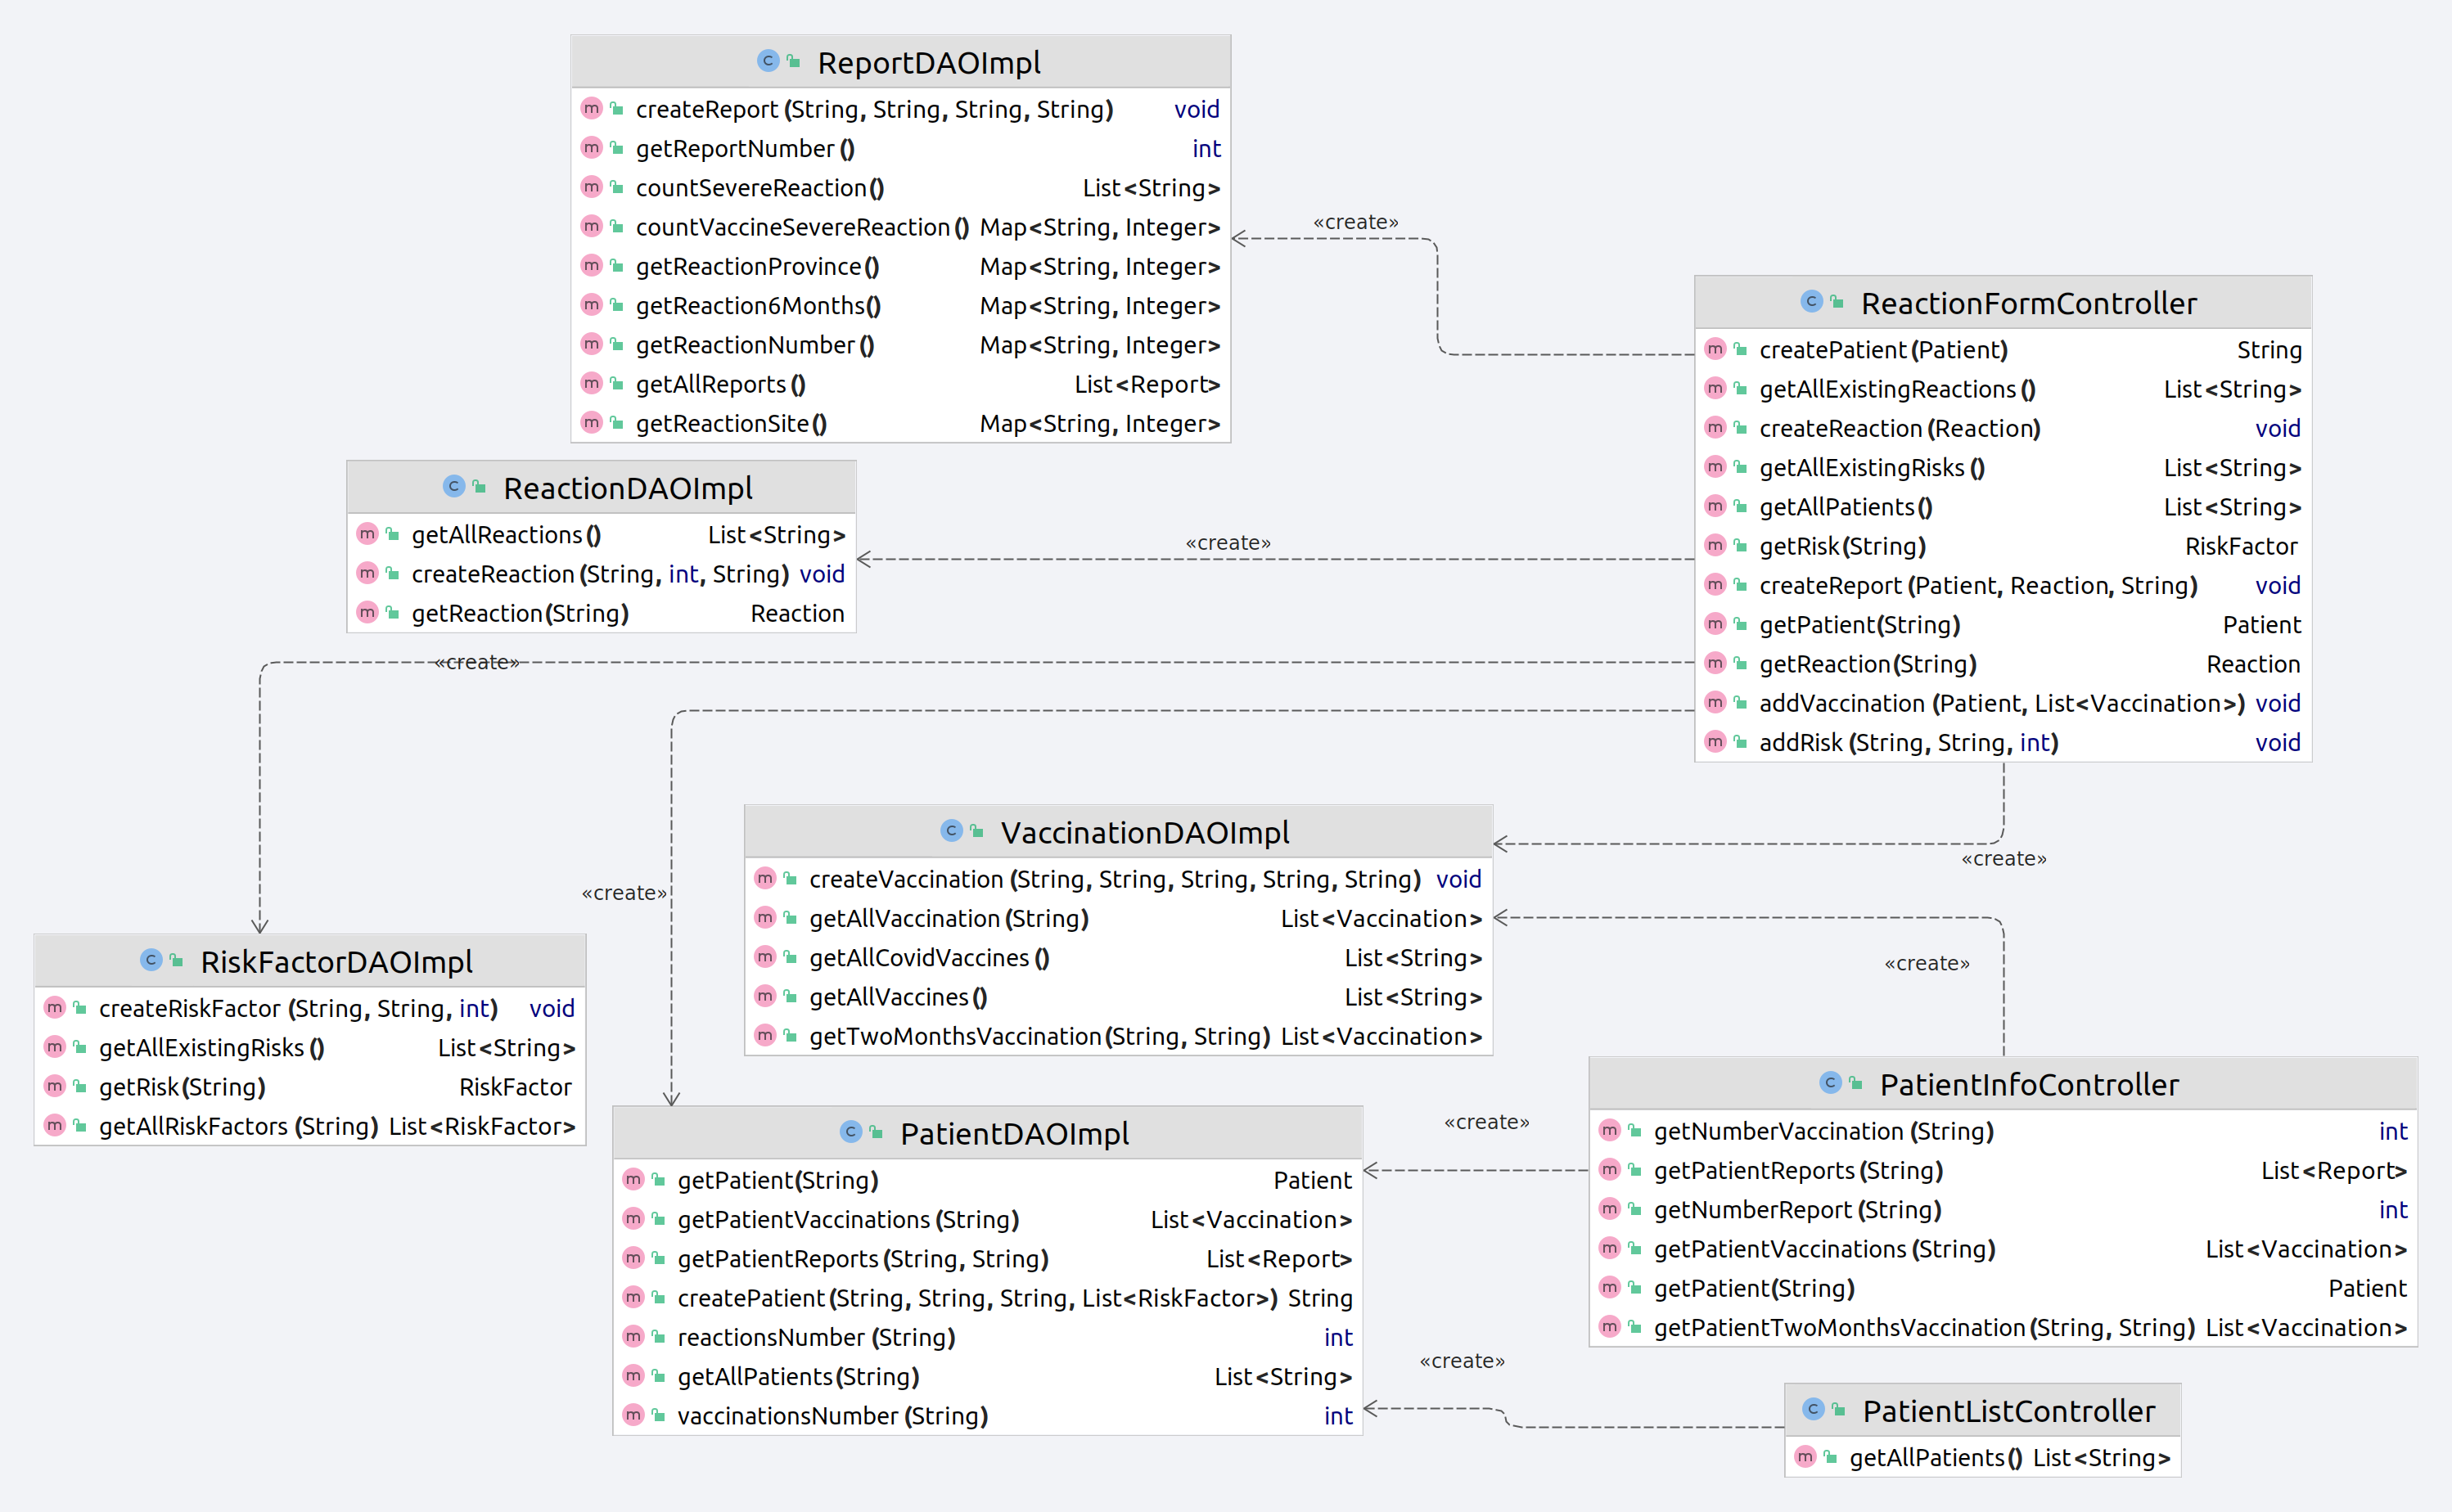
\includegraphics[width=1\textwidth]{pictures/ControllerDati.png}
                \captionof{figure}{Interazione tra le classi del Controller del Dottore e i dati a cui ha accesso}
                \end{center}

    \newpage
        \subsection{Sequence Diagram}
            \subsubsection*{Chiamate della View del PatientInfo nel metodo getView}
            \begin{center}
                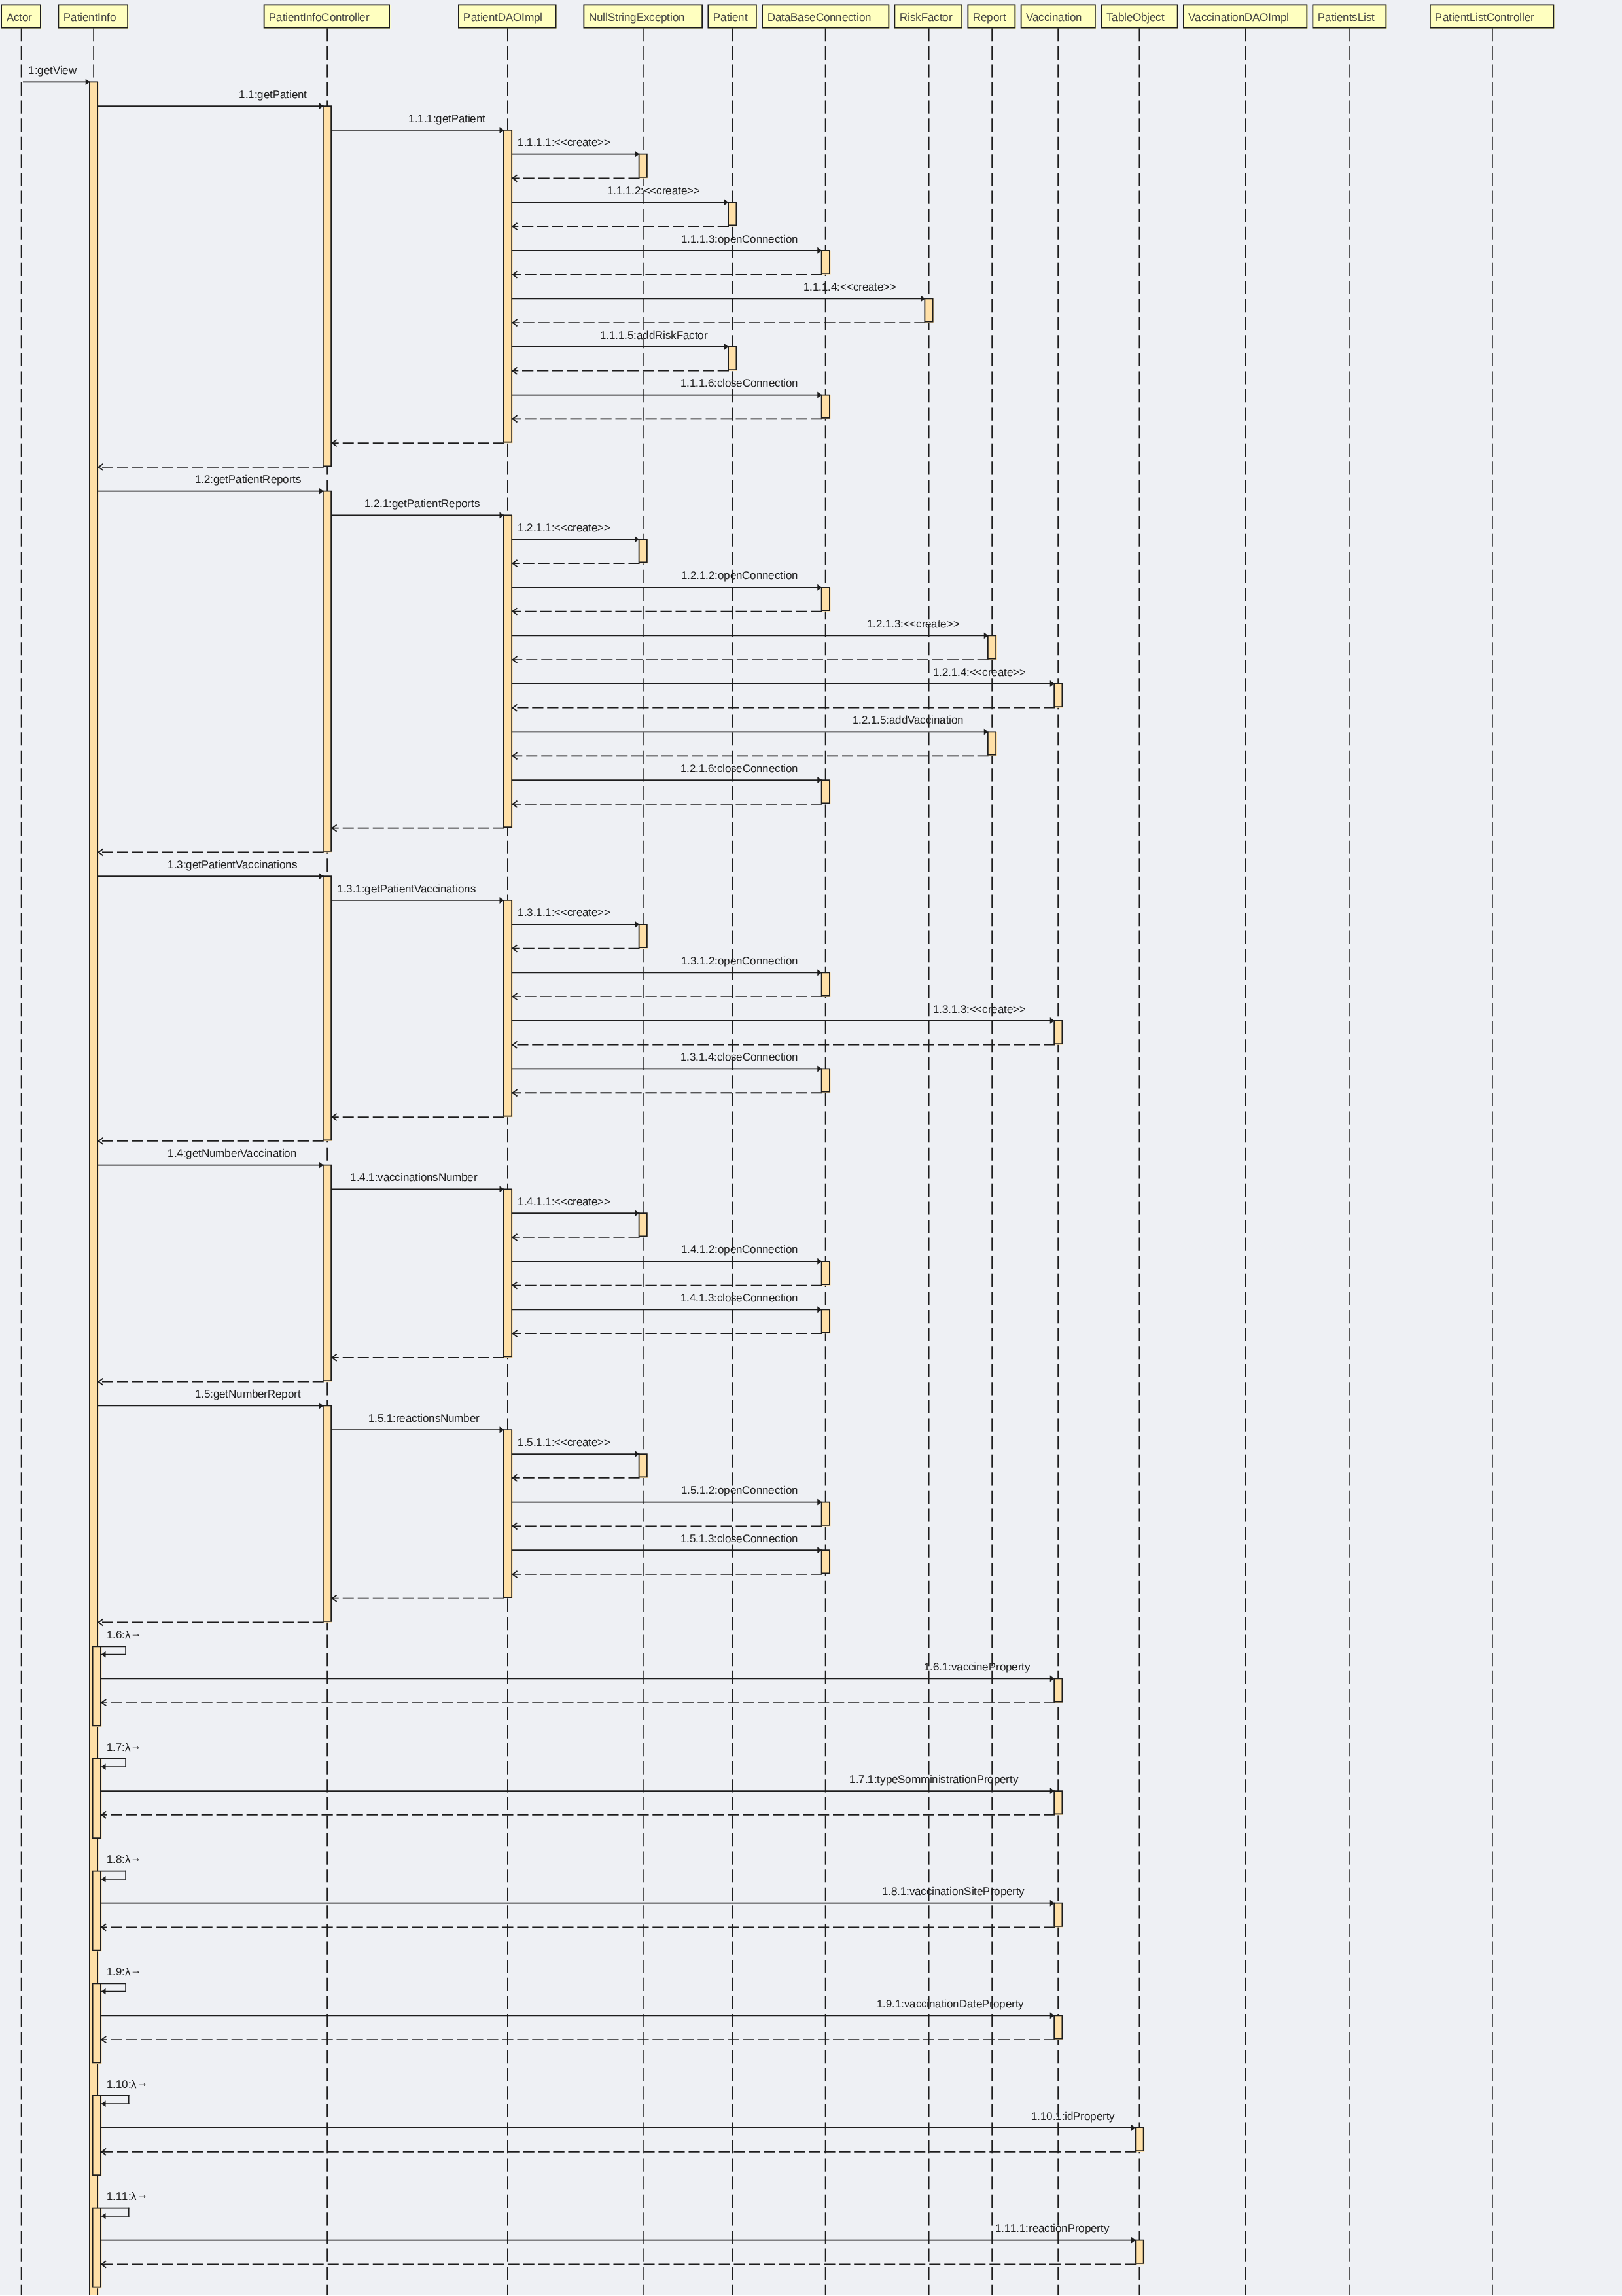
\includegraphics[width=0.90\textwidth]{pictures/prova_001.png}
            \end{center}
    \newpage
        \begin{center}
            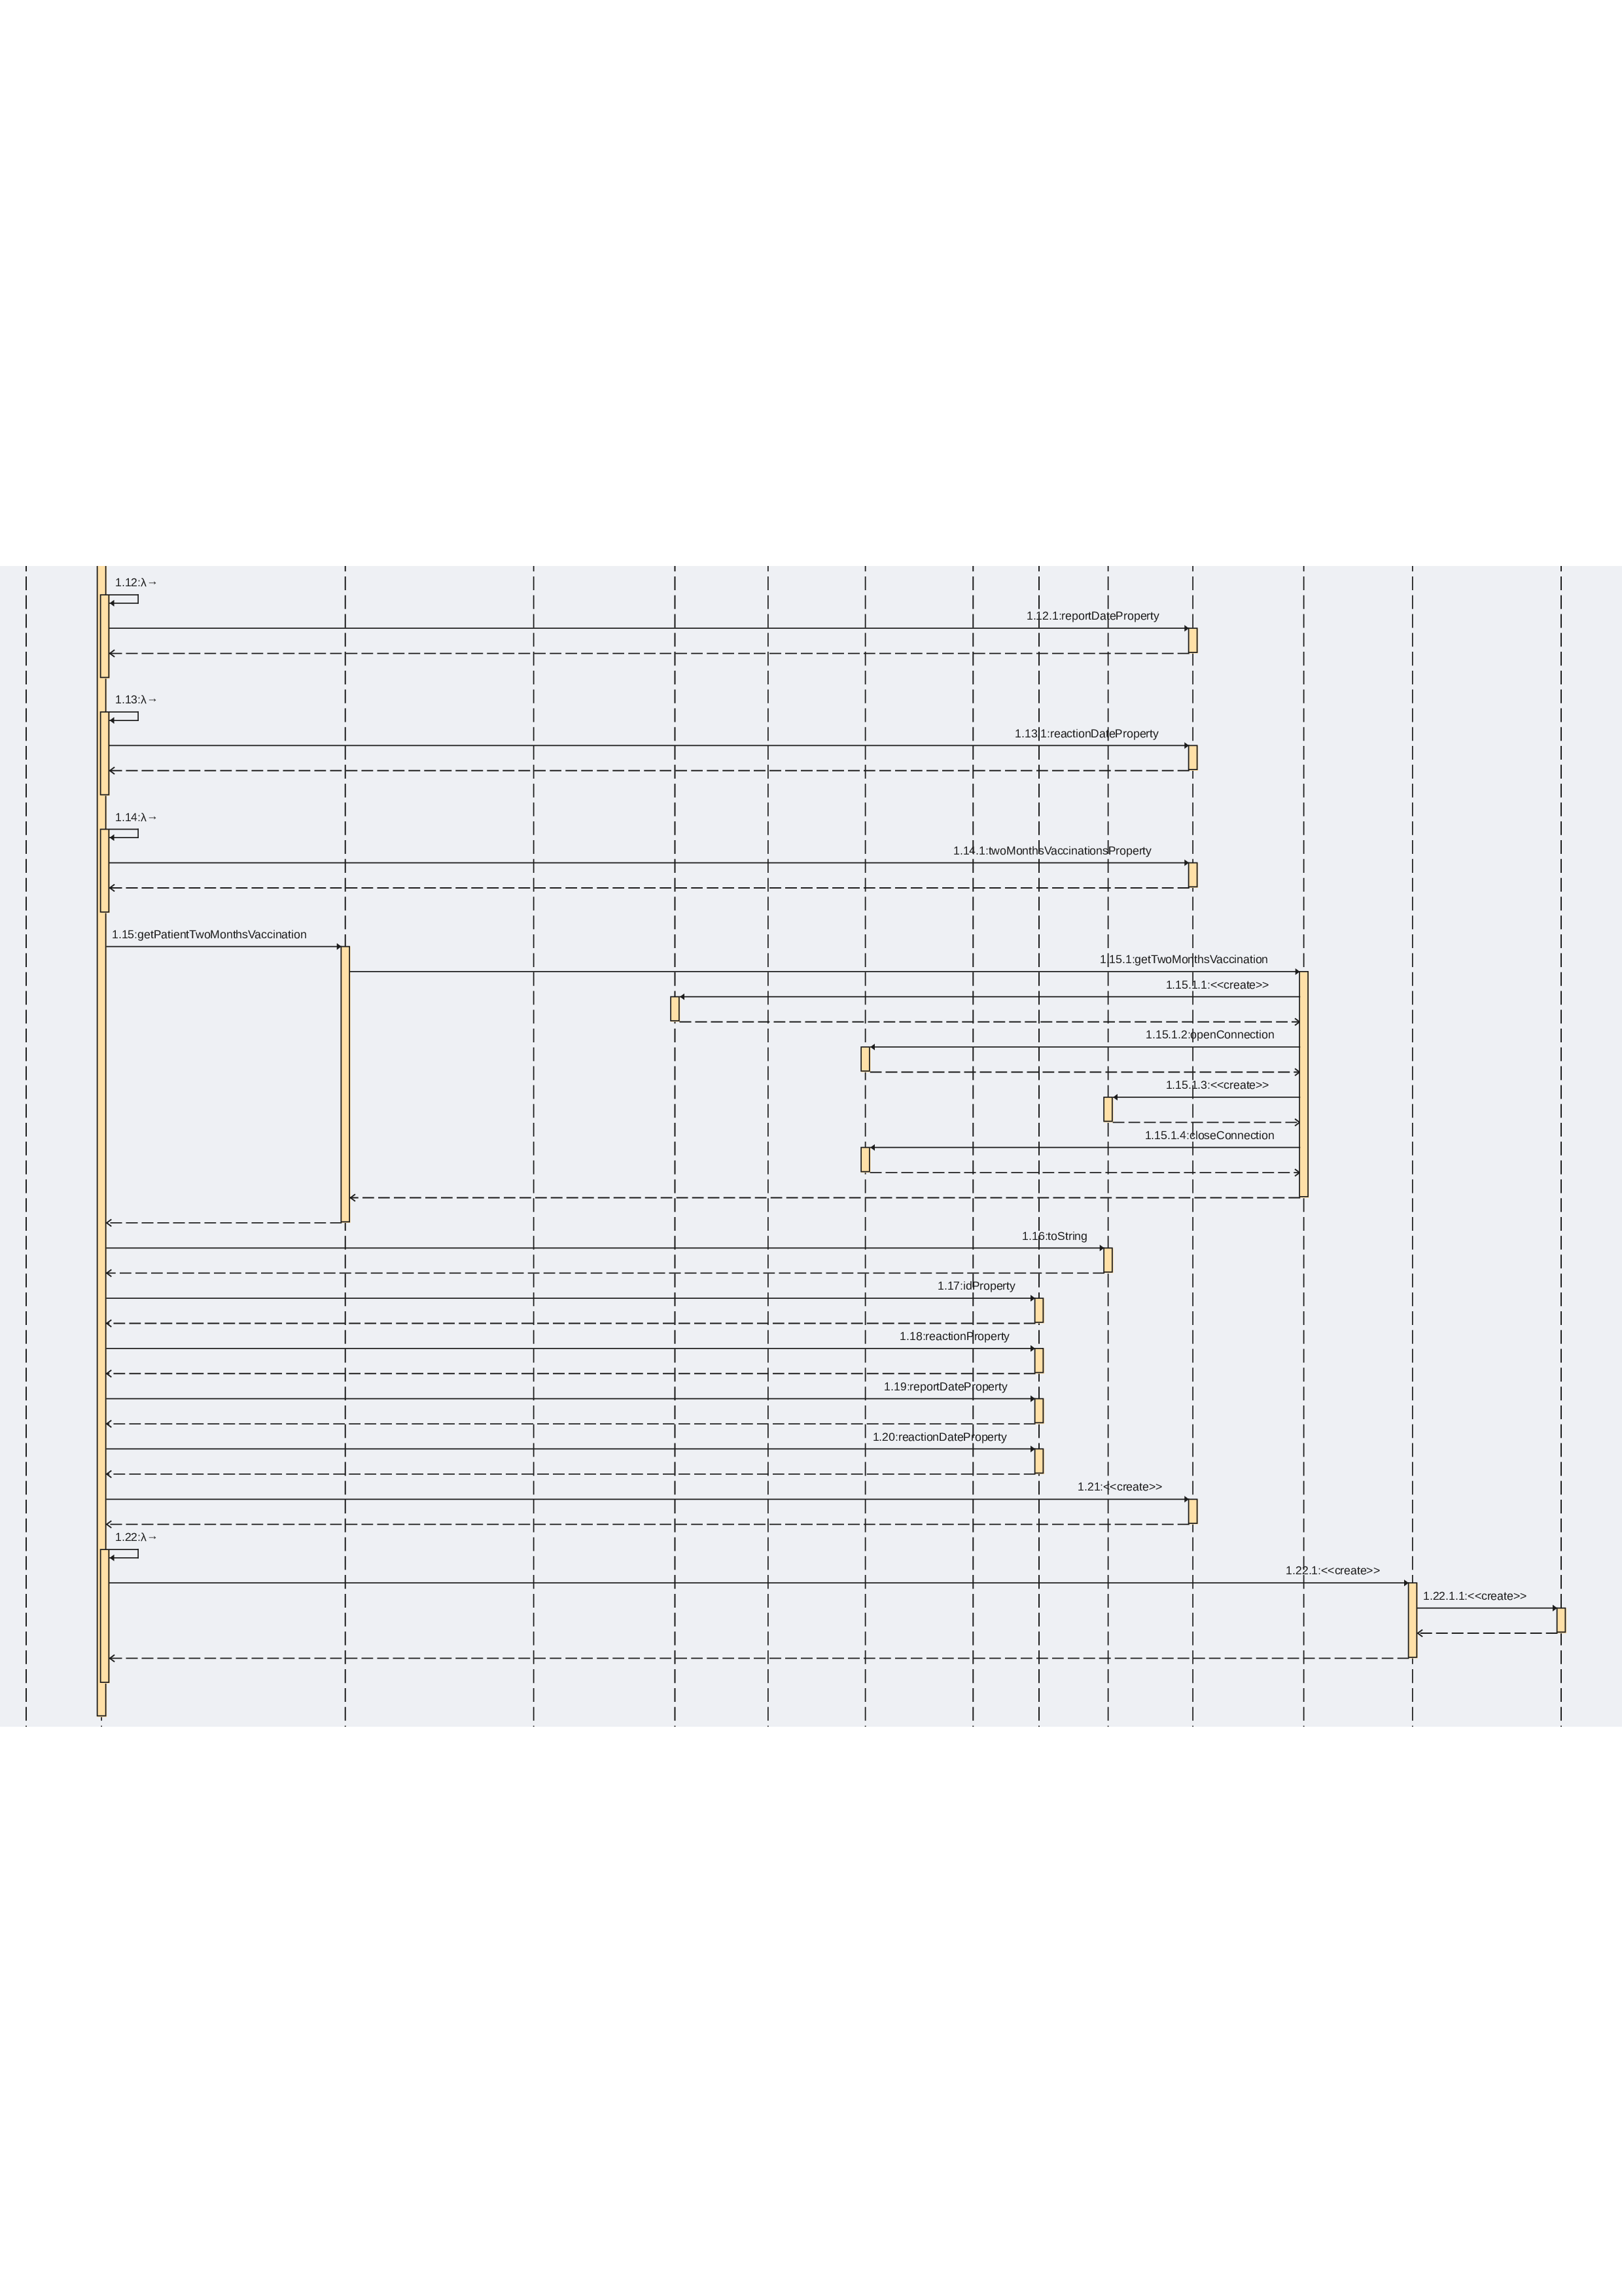
\includegraphics[width=0.90\textwidth]{pictures/prova_002.png}
        \end{center}
    \newpage
        \subsubsection*{Chiamate della View del ControlPhaseForm nel metodo getView}
        \begin{center}
            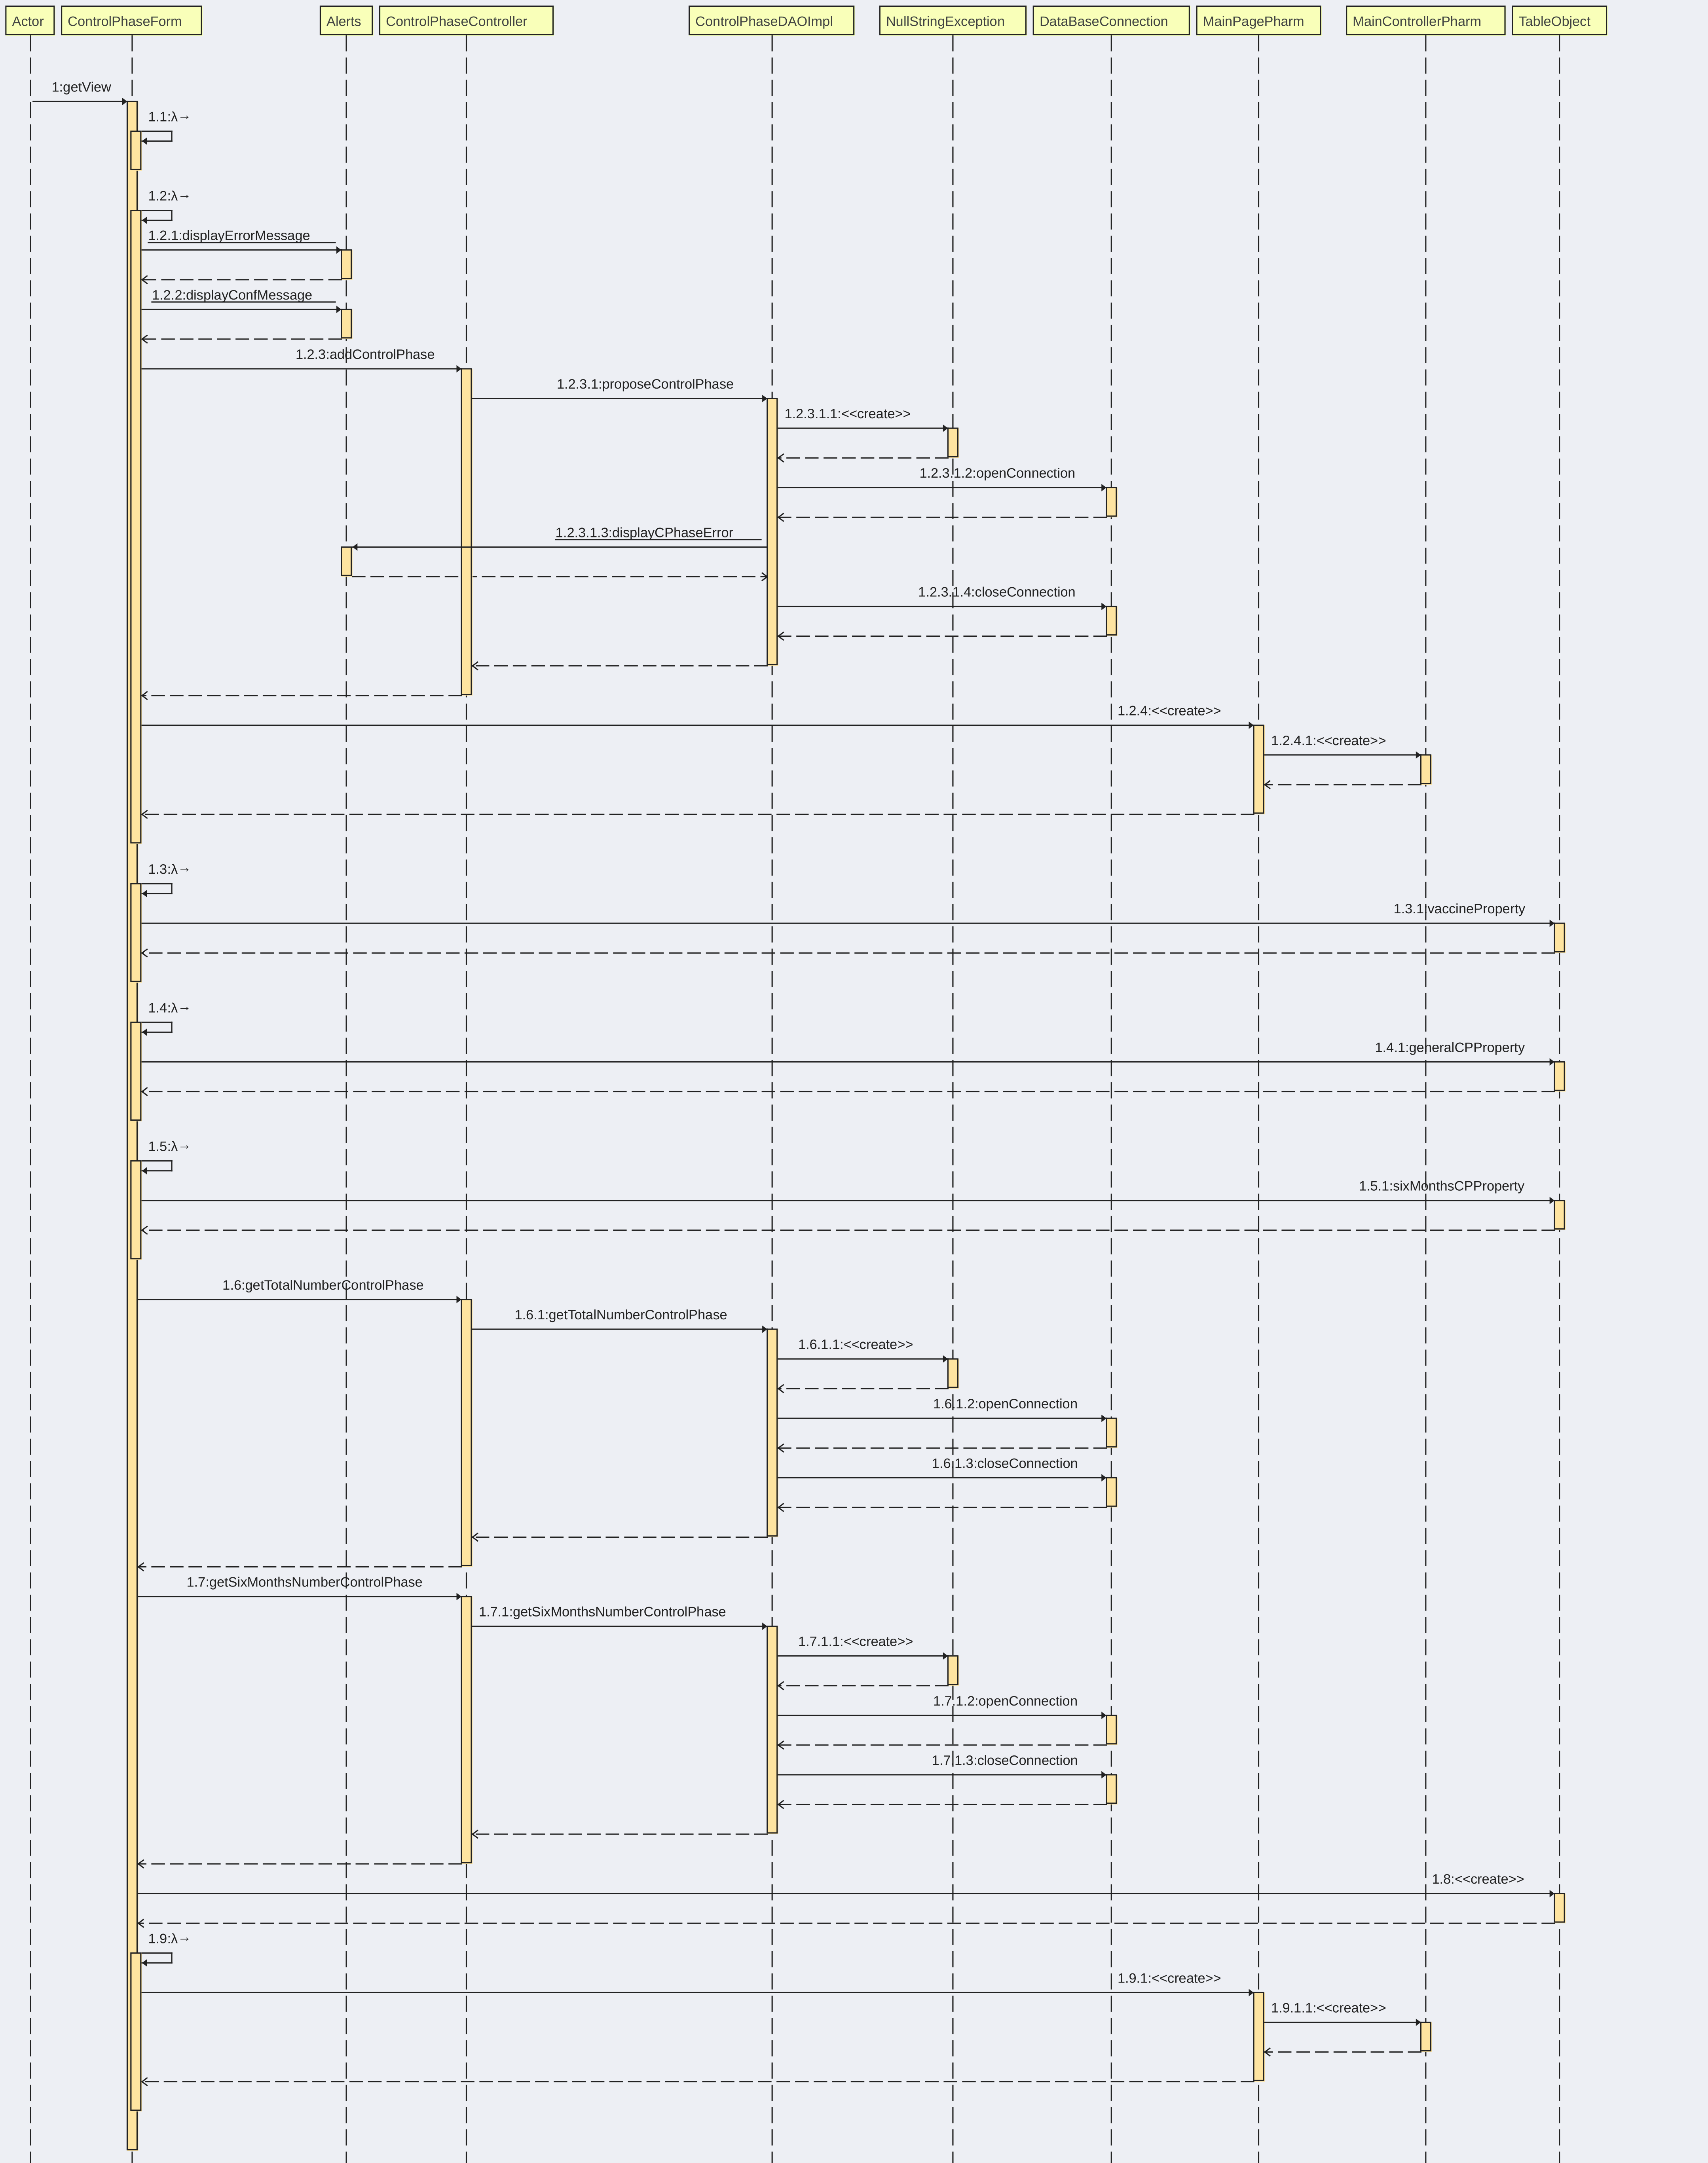
\includegraphics[width=1\textwidth]{pictures/prova.png}
        \captionof{figure}{}
        \end{center}

    \newpage
    \section{Implementazione del DataBase}
    Come richiesto dalla traccia si è implementato un database con cui l'applicazione potesse interagire.\\
    Il Database è stato creato sulla base dell'ER qui riportato:
        \begin{center}
            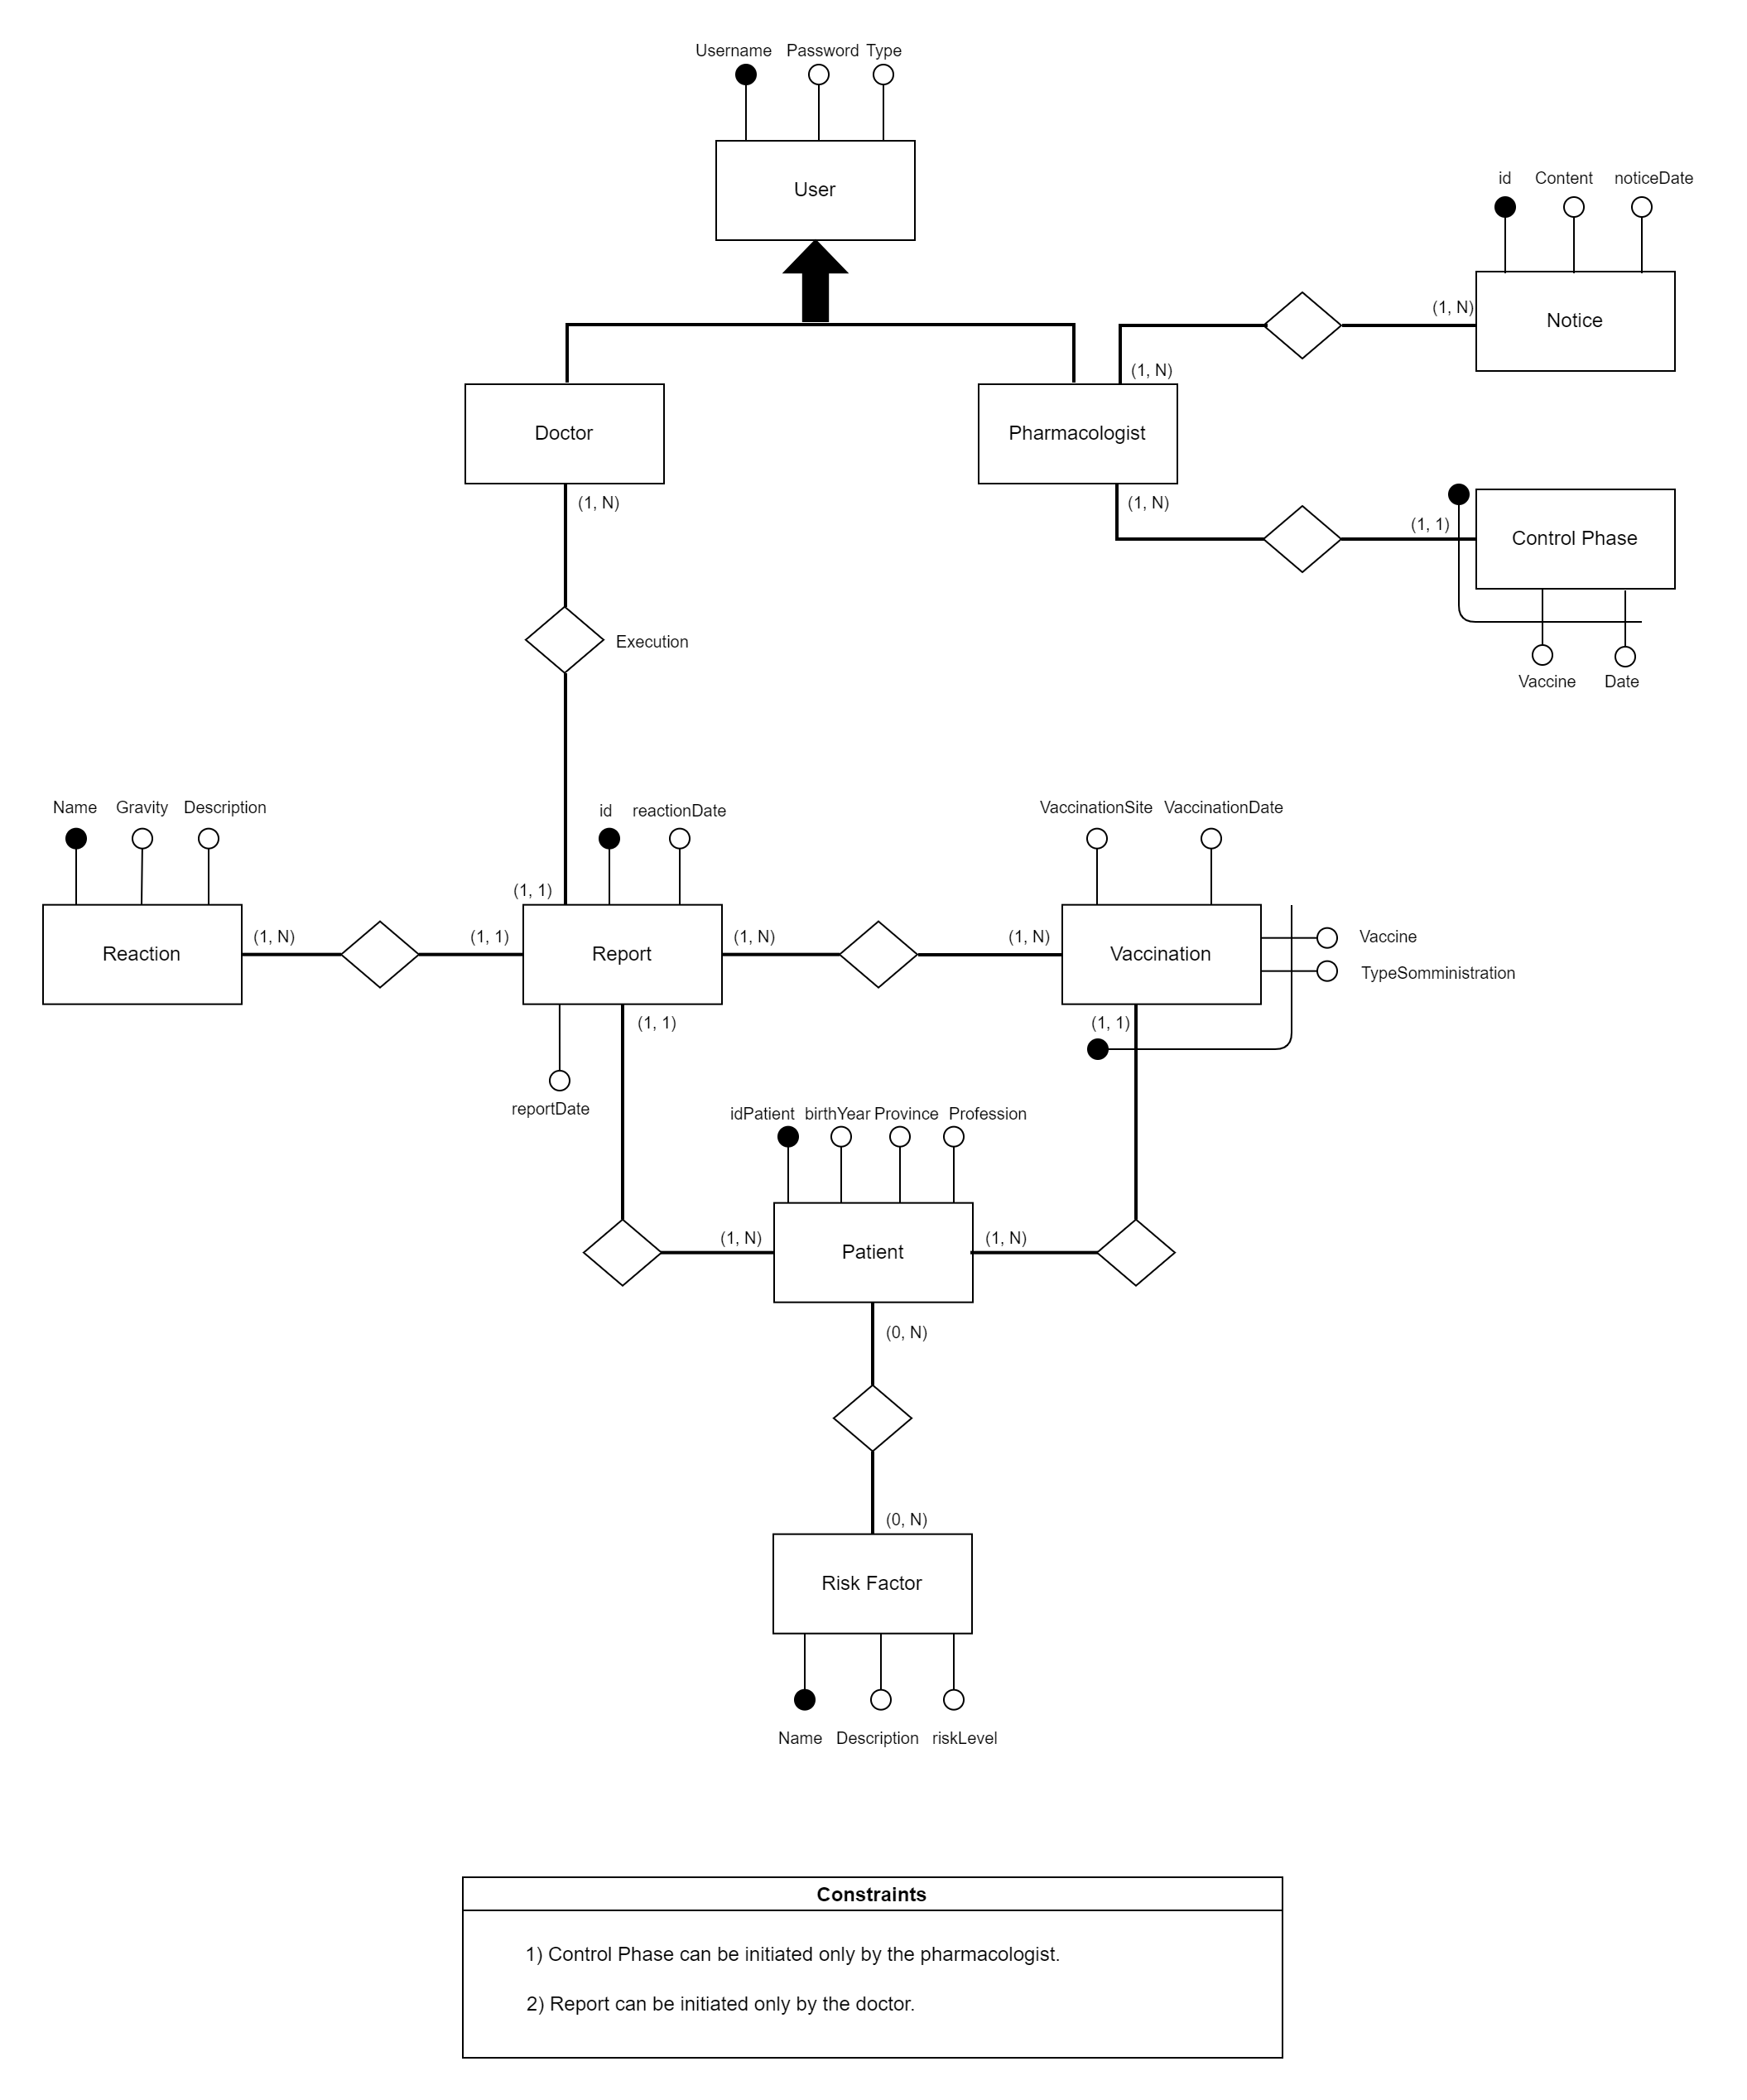
\includegraphics[width=1\textwidth]{pictures/Schema_ER.png}
            \captionof{figure}{Schema ER}
        \end{center}
    Modello relazionale:
    \begin{itemize}
        \item ControlPhase (\underline{Pharmacologist}, \underline{Vaccine}, \underline{Date})
        \item Notice (\underline{Id}, Content, noticeDate)
        \item Patient (\underline{idPatient}, birthYear, Province, Profession)
        \item PatientRisk (\underline{idPatient}, \underline{Risk})
        \item ReadNotice (\underline{noticeId}, \underline{pharmId})
        \item Report (\underline{Id}, reportDate, reactionDate, Reaction, idPatient, Doctor)
        \item RiskFactor (\underline{Name}, Description, RiskLevel)
        \item Users (\underline{Username}, Password, Type)
        \item Vaccination (\underline{idPatient}, \underline{Vaccine}, \underline{typeSomministration}, vaccinationSite, vaccinationDate)
    \end{itemize}

    Vincoli di chiave esterna:
        \begin{itemize}
            \item ControlPhase.pharmacologist \textrightarrow Users
            \item PatientRisk.idpatient \textrightarrow Patient
            \item ReadNotice.noticeid \textrightarrow Notice
            \item ReadNotice.pharmid \textrightarrow Users
            \item Report.reaction \textrightarrow Reaction
            \item Report.idpatient \textrightarrow Patient
            \item Report.doctor \textrightarrow Users
            \item Vaccination.idpatient \textrightarrow Patient
        \end{itemize}

    A livello implementativo nell'applicazione, le chiavi esterne riferite a Users si riferiscono a utenti di tipologie diverse:
        \begin{itemize}
            \item ControlPhase.pharmacologist fa riferimento ad uno user farmacologo (User.type = 1)
            \item ReadNotice.pharmid fa riferimento ad uno user farmacologo (User.type = 1)
            \item Report.doctor fa riferimento ad uno user medico (User.type = 0)
        \end{itemize}

\newpage
    \section{Fase di Test}
    Il test dell'applicazione è stato iniziato in concomitanza con il termine del primo prototipo, in accordo con la metodologia di sviluppo Plan-Driven adottata.\\
    Si è divisa la fase di test in 4 fasi principali:
        \begin{enumerate}
            \item Verifica interna della consistenza dell'applicazione rispetto all'analisi dei requisiti.
            \item \textbf{Test di sviluppo}, implementati come unit test automatizzati mediante JUnit per verificare la correttezza di
            alcune delle classi più problematiche.
            \item \textbf{Test di release}, consistente in alcuni stress test, con un team simulato di colleghi esterni allo sviluppo dell'applicazione.
            \item \textbf{Test degli utenti}, in cui si è scelto un campione di conoscenti senza background informatico che verificassero il software facendo le veci di utenti reali in situazioni reali.
        \end{enumerate}
    
        \subsubsection*{Nota}
        Il primo prototipo è da intendersi come la prima versione con tutte le features implementate ma senza aver passato il testing, ultimata in data 21/06/2022.

        \subsection{Test di Sviluppo: Unit Test}
        Per la parte di Test di sviluppo si è scelto di implementare degli Unit Test sulle classi del \textbf{Controller}. Questa scelta è derivata dal fatto che il controller rappresenta l'interazione tra l'interfaccia (testabile a livello visuale) e le DAO (le cui funzioni sono utilizzate dai controller e quindi implicitamente testate.)\\
            \begin{itemize}
                \item Per ogni calsse del controller ed ogni metodo si è scelto di \textbf{testare la normale funzione}: input normali con il confronto dei risultati rispetto a quelli che ci si aspetta dall'implementazione e popolazione del DataBase. Per questo la fase di testing unitario è stata statica e ha riguardato una sola giornata di lavoro, successivamente al termine del primo propototipo.
                \item Per ogni metodo si è implementato anche un test che verificasse l'\textit{handling} degli errori all'interno delle classi. Dando in input oggetti o stringhe vuote si è verificato che i metodi non ritornassero alcuna informazione, o stampassero in \textbf{Standard Output} o \textbf{Standard Error} i messaggi di errore impostati nei catch delle eccezioni.
            \end{itemize}
        Tutte le classi di test hanno ottenuto un buon risultato, i metodi per cui sono stati rilevati errori (ad esempio non stampavano il messaggio esatto) sono state ricontrollati e corretti. Ogni test è visibile nella sezione apposita dell'eseguibile.
        
        \subsubsection*{Nota}
        Al termine delle Unit Test definiamo ora l'applicazione come la \textbf{release 1.0}, "rilasciata" in data 24/06/2021. Questa verrà sottoposta ai test di release.

    \newpage
        \subsection{Test di release}
        Per effettuare i test di release si è deciso di trovare 4 colleghi disposti a testare l'applicazione e ad effettuare gli \textbf{stress test} che ritenessero più adeguati.\\
        In data 25/06/2022 l'applicazione è stata sottoposta a testing, riportiamo le considerazioni dei \textit{tester}:
            \begin{itemize}
                \item 
            \end{itemize}

    \newpage
        \subsection{Test degli utenti}
        In questo caso si è deciso di simulare un test dell'utente che fosse il più possibile vicino ad un vero test: si sono scelti 3 \textit{tester senza background informatico}.\\
        Ai tester si è richiesto di eseguire il test di alcune funzionalità all'interno dell'applicazione.
            \begin{itemize}
                \item Il primo tester ha fatto le veci di un nuovo utente Dottore, non inizializzato, che non avesse quindi nessun paziente inserito a database. Gli si è chiesto, oltre al testare le normali funzionalità, di inserire nello specifico: un nuovo paziente con una nuova reazione e una nuova storia vaccinale, e successivamente per lo stesso paziente (quindi già esistente)
                di inserire una seconda reazione, questa volta esistente e di aggiungere una vaccinazione alla storia.\footnote{Si veda l'appendice B, alla sezione "Passi che si richiede di effettuare, Tester 1}
                \item Il secondo tester ha fatto le veci di un utente Dottore già esistente, quindi con pazienti già inseriti. Gli si è chiesto di inserire: un nuovo paziente con una reazione già esistente e in seguito di aggiungere, per un paziente già esistente, una nuova reazione.\footnote{Si veda l'appendice B, alla sezione "Passi che si richiede di effettuare, Tester 2}
            \end{itemize}
        In questo modo si sono testate tutte le combinazioni di inserimento dei report da parte dei dottori. Alla fine dei test è stato somministrato un questionario, in cui si è chiesto di valutare (positivamente o negativamente) le diverse funzionalità testate nella parte "Dottore".\footnote{Si veda l'appendice C: Questionari}
            \begin{itemize}
                \item Il terzo tester ha fatto le veci di un nuovo utente Farmacologo, con tutti gli avvisi generati ancora da leggere e una fase di controllo da proporre. \footnote{Si veda l'appendice B, alla sezione "Passi che si richiede di effettuare, nella sezione farmacologo"}
            \end{itemize}
        Anche in questo caso alla fine sono stati somministrati i questionari di valutazione.
    Al termine si sono anche raccolti a voce suggerimenti e note, che riportiamo: 
    \paragraph*{Considerazioni dei tester}
\newpage
    \section*{Appendice A: Query di creazione Database}
    \addcontentsline{toc}{section}{Appendice A: DataBase}

    Si è scelto di implementare il Database in PostgreSQL. Riportiamo anche le query usate per la creazione delle tabelle, che ci aiutano a comprendere com'è fatto:
    \paragraph*{Tabelle dello schema VaccineSupervisionDB}
        \begin{verbatim}
        CREATE TABLE patient(
            idPatient SERIAL PRIMARY KEY,
            birthYear NUMERIC(4) NOT NULL ,
            CHECK ( birthYear >= 1900 ),
            province VARCHAR(20) NOT NULL,
            profession VARCHAR(50) NOT NULL
        );
        
        CREATE TABLE RiskFactor(
            name VARCHAR(50) PRIMARY KEY,
            description VARCHAR(50),
            riskLevel NUMERIC(1) NOT NULL,
            CHECK ( riskLevel >= 1 AND riskLevel <= 5 )
        );
        
        CREATE TABLE Vaccination(
            idPatient INTEGER REFERENCES patient(idPatient),
            vaccine VARCHAR(50) NOT NULL,
            typeSomministration VARCHAR(25) NOT NULL,
            PRIMARY KEY (idPatient, vaccine, typeSomministration),
            vaccinationSite VARCHAR(25) NOT NULL,
            vaccinationDate DATE NOT NULL
        );
        
        CREATE TABLE Reaction(
            name VARCHAR(20) PRIMARY KEY,
            gravity NUMERIC(1) NOT NULL,
            CHECK(gravity >= 1 AND gravity <= 5),
            description VARCHAR(50) NOT NULL
        );
        
        CREATE TABLE PatientRisk(
            idPatient INTEGER NOT NULL REFERENCES patient(idPatient),
            risk VARCHAR(20) NOT NULL REFERENCES RiskFactor(name),
            PRIMARY KEY(idPatient, risk)
        );
        
        CREATE TABLE users(
            username VARCHAR(10) PRIMARY KEY,
            password VARCHAR(12) NOT NULL,
            type BOOLEAN NOT NULL,
            UNIQUE (username, password)
        );
        
        CREATE TABLE Report(
            id SERIAL PRIMARY KEY,
            reportDate DATE NOT NULL DEFAULT CURRENT_DATE,
            reactionDate DATE NOT NULL,
            reaction VARCHAR(20) NOT NULL REFERENCES Reaction(name),
            idPatient INTEGER NOT NULL REFERENCES patient(idPatient),
            doctor VARCHAR(10) REFERENCES users(username)
        );
        
        CREATE TABLE ControlPhase(
            pharmacologist VARCHAR(10) REFERENCES users(username),
            vaccine VARCHAR(15) NOT NULL,
            date DATE NOT NULL,
            PRIMARY KEY (pharmacologist, vaccine, date)
        );
        \end{verbatim}
    
    \newpage
    \section*{Appendice B: Documento per i tester}
    \addcontentsline{toc}{section}{Appendice B: Test Utente}

    \section*{Test dell'utente Dottore}

        \subsection*{Traccia su cui basare l'idea del funzionamento}
            Di seguito riportiamo la traccia dell'elaborato per quel che riguarda le funzionalità dell'utente di tipo Dottore.
            \begin{quotation}
                Si vuole progettare un sistema software per gestire le segnalazioni di reazioni avverse (ad esempio, asma, dermatiti, insufficienza renale, miocardiopatia, \dots) da vaccini anti-Covid.\\
                Ogni segnalazione è caratterizzata da un codice univoco, dall'indicazione del paziente a cui fa riferimento, dall'indicazione della reazione avversa, dalla data della reazione avversa, dalla data di segnalazione, e dalle vaccinazioni ricevute nei due mesi precedenti il momento della reazione avversa.
                Per ogni paziente sono memorizzati: un codice univoco, l'anno di nascita, la provincia di residenza e la professione.\\
                Per ogni paziente è possibile memorizzare gli eventuali fattori di rischio presenti (paziente fumatore, iperteso, sovrappeso, paziente fragile per precedenti patologie cardiovascolari o oncologiche), anche più d'uno. Ogni fattore di rischio è caratterizzato da un nome univoco, una descrizione e il livello di rischio associato. Per ogni paziente è, inoltre, memorizzata l'intera storia delle sue vaccinazioni precedenti, anti-Covid-19 e antinfluenzali.\\
                Ogni vaccinazione è caratterizzata da: paziente a cui si riferisce, segnalazioni a cui è legata, vaccino somministrato (AstraZeneca, Pfizer, Moderna, Sputnik, Sinovac, antinfluenzale, \dots), tipo della somministrazione (I, II, III o IV dose, dose unica), sede presso la quale è avvenuta la vaccinazione e data di vaccinazione. Per ogni reazione avversa sono memorizzati un nome univoco, un livello di gravità (da 1 a 5) e una descrizione generale, espressa in linguaggio naturale. Una reazione avversa può essere legata a molte segnalazioni. Per ogni paziente sono memorizzati il numero di reazioni avverse segnalate ed il numero di vaccinazioni ricevute.\\
                Il sistema deve supportare i medici che effettuano la segnalazione. \textbf{Dopo opportuna autenticazione, il medico viene introdotto ad una interfaccia che permette l'inserimento dei dati delle reazioni avverse e dei pazienti. Il codice univoco dei pazienti è gestito dal sistema, che tiene traccia dei pazienti indicati da ogni medico. Ogni medico vede solo i codici identificativi dei pazienti, dei quali ha già segnalato qualche reazione avversa, e le relative informazioni.}
            \end{quotation}

        \subsection*{Passi che si richiede di effettuare}

            \subsubsection*{Tester 1}
            Dopo aver avviato l'applicazione si chiede all'utente di effettuare i seguenti passaggi:
            \begin{enumerate}
                \item Effettuare un login tramite le credenziali: username=\textit{doc12}, password=\textit{PROVA}.
                \item Verificare che l'accesso è negato.
                \item Effettuare un login tramite le credenziali: username=\textit{doc3}, password=\textit{DOC3}.
                \item Verificare che l'accesso è eseguito come dottore.
                \item Accedere alla lista pazienti tramite l'apposito bottone.
                \item Verificare che questa sia vuota.
                \item Tornare alla pagina principale.
                \item Accedere al form di inserimento dei report
                \item Nella prima tab cliccare il bottone di inserimento di un nuovo paziente.
                \item Inserire le seguenti informazioni\\
                        Anno di nascita: \textit{1959}, Provincia: \textit{Lecco}, Professione:\textit{Impiegato}, scegliere tra i fattori di rischio il fattore esistente \textit{Colesterolo alto}.
                \item Passare alla tab successiva e inserire come data reazione, dall'apposito calendario il \textit{22 Maggio del 2022}.
                \item Cliccare il bottone di inserimento di una nuova reazione.
                \item Inserire le seguenti informazioni\\ 
                        Nome: \textit{Trombosi}, Descrizione: \textit{Presenza di un coagulo di sangue, che aderisce alle pareti non lesionate dei vasi.}, Gravità: \textit{4}.
                \item Passare alla tab successiva e scegliere dai vaccini: \textit{Antinfluenzale A/Victoria/2570/2019}
                \item Inserire nei campi di testo:\\
                        Sito della vaccinazione: \textit{Varenna}, Data della vaccinazione: \textit{4/12/2022}
                \item Cliccare su inserisci.
                \item Inserire nuovamente un vaccino: questa volta si scelga il vaccino \textit{Pfizer}
                \item Apparirà un nuovo bottone per scegliere il tipo di somministrazione, si clicchi su: \textit{Prima dose}
                \item Inserire nei campi di testo:\\
                    Sito della vaccinazione: \textit{Varenna}, Data della vaccinazione: \textit{2/16/2022}
                \item Cliccare su inserisci.
                \item Inserire nuovamente un vaccino: questa volta si scelga il vaccino \textit{Moderna}
                \item Apparirà un nuovo bottone per scegliere il tipo di somministrazione, si clicchi su: \textit{Seconda dose}
                \item Inserire nei campi di testo:\\
                    Sito della vaccinazione: \textit{Lecco}, Data della vaccinazione: \textit{4/31/2022}
                \item Cliccare su inserisci.
                \item Cliccare su conferma.
                \item Apparirà ora un avviso di conferma, cliccare su OK.
                \item Si tornerà sutomaticamente nella pagina iniziale. 
                \item Accedere alla lista pazienti tramite l'apposito bottone.
                \item Verificare la presenza di un nuovo paziente
                \item Cliccare sul bottone "Info".
                \item Dalla pagina aperta scorrere tra le tab e verificare la correttezza delle informazioni inserite.
                \item Tornare indietro e poi ancora fino alla pagina principale.
                \item Accedere di nuovo al form di inserimento dei report.
                \item Selezionare il paziente già esistente nella prima tab.
                \item Inserire come data della reazione: \textit{15 Giugno 2022}
                \item Selezionare dalle reazioni esistenti la reazione \textit{Eruzione cutanea}
                \item Nella tab successiva, inserire una nuova vaccinazione:\\
                    si scelga il vaccino \textit{Moderna}
                \item Apparirà un nuovo bottone per scegliere il tipo di somministrazione, si clicchi su: \textit{Dose booster}
                \item Inserire nei campi di testo:\\
                    Sito della vaccinazione: \textit{Varenna}, Data della vaccinazione: \textit{6/3/2022}
                \item Cliccare su conferma.
                \item Verificare nuovamente le informazioni inserite dalla pagina di visualizzazione dei pazienti.
                \item Tornare alla pagina iniziale.
                \item Effettuare il logout.
            \end{enumerate}

            \subsubsection*{Tester 2}
            Dopo aver avviato l'applicazione si chiede all'utente di effettuare i seguenti passaggi:
            \begin{enumerate}
                \item Effettuare un login tramite le credenziali: username=\textit{doc2}, password=\textit{PROVA}.
                \item Verificare che l'accesso è negato.
                \item Effettuare un login tramite le credenziali: username=\textit{doc1}, password=\textit{DOC1}.
                \item Verificare che l'accesso è eseguito come dottore.
                \item Accedere alla lista pazienti tramite l'apposito bottone.
                \item Verificare che questa sia popolata.
                \item Tornare alla pagina principale.
                \item Accedere al form di inserimento dei report
                \item Nella prima tab cliccare il bottone di inserimento di un nuovo paziente.
                \item Inserire le seguenti informazioni\\
                        Anno di nascita: \textit{1980}, Provincia: \textit{Salerno}, Professione:\textit{Ristoratore}, 
                        inserire un nuovo fattore di rischio: Nome: \textit{Sovrappeso}, Descrizione: \textit{Paziente con un peso superiore a quello indicato per eta e statura}, Livello di rischio: \textit{3}. Cliccare il bottone di inserimento.
                \item Selezionare ora il fattore di rischio aggiunto dal menù a tendina.
                \item Passare alla tab successiva e inserire come data reazione, dall'apposito calendario il \textit{30 Maggio del 2022}.
                \item Selezionare dalle reazioni esistenti la reazione \textit{Vomito}
                \item Passare alla tab successiva e scegliere dai vaccini: \textit{Antinfluenzale A/Darwin/6/2021}
                \item Inserire nei campi di testo:\\
                        Sito della vaccinazione: \textit{Salerno}, Data della vaccinazione: \textit{5/20/2022}
                \item Cliccare su inserisci.
                \item Inserire nuovamente un vaccino: questa volta si scelga il vaccino \textit{Jannsen}
                \item Apparirà un nuovo bottone per scegliere il tipo di somministrazione, si clicchi su: \textit{Unica}
                \item Inserire nei campi di testo:\\
                    Sito della vaccinazione: \textit{Salerno}, Data della vaccinazione: \textit{4/16/2022}
                \item Cliccare su inserisci.
                \item Cliccare su conferma.
                \item Apparirà ora un avviso di conferma, cliccare su OK.
                \item Si tornerà sutomaticamente nella pagina iniziale. 
                \item Accedere alla lista pazienti tramite l'apposito bottone.
                \item Verificare la presenza di un nuovo paziente
                \item Cliccare sul bottone "Info".
                \item Dalla pagina aperta scorrere tra le tab e verificare la correttezza delle informazioni inserite.
                \item Tornare indietro e poi ancora fino alla pagina principale.
                \item Accedere di nuovo al form di inserimento dei report.
                \item Selezionare il paziente con codice 20 nella prima tab.
                \item Inserire come data della reazione: \textit{23 Giugno 2022}
                \item Cliccare il bottone di inserimento di una nuova reazione.
                \item Inserire le seguenti informazioni\\ 
                        Nome: \textit{Dermatite}, Descrizione: \textit{Infiammazione della pelle causata dalla reazione a determinate sostanze chimiche o naturali (dette allergeni).}, Gravità: \textit{2}.
                \item Nella tab successiva, inserire una nuova vaccinazione:\\
                    si scelga il vaccino \textit{Moderna}
                \item Apparirà un nuovo bottone per scegliere il tipo di somministrazione, si clicchi su: \textit{Dose booster}
                \item Inserire nei campi di testo:\\
                    Sito della vaccinazione: \textit{Torino}, Data della vaccinazione: \textit{6/20/2022}
                \item Cliccare su conferma.
                \item Verificare nuovamente le informazioni inserite dalla pagina di visualizzazione dei pazienti.
                \item Tornare alla pagina iniziale.
                \item Effettuare il logout.
            \end{enumerate}

        \subsection*{Tabella di valutazione}
            Si chiede ad entrambi i partecipanti di compilare la tabella di valutazione data assieme a questo modulo.

    \newpage
        \section*{Test dell'utente Farmacologo}
            \subsection*{Traccia su cui basare l'idea del funzionamento}
            Di seguito riportiamo la traccia dell'elaborato per quel che riguarda le funzionalità dell'utente di tipo Dottore.
            \begin{quotation}
            Si vuole progettare un sistema software per gestire le segnalazioni di reazioni avverse (ad esempio, asma, dermatiti, insufficienza renale, miocardiopatia, \dots) da vaccini anti-Covid.\\
                Ogni segnalazione è caratterizzata da un codice univoco, dall'indicazione del paziente a cui fa riferimento, dall'indicazione della reazione avversa, dalla data della reazione avversa, dalla data di segnalazione, e dalle vaccinazioni ricevute nei due mesi precedenti il momento della reazione avversa.
                Per ogni paziente sono memorizzati: un codice univoco, l'anno di nascita, la provincia di residenza e la professione.\\
                Per ogni paziente è possibile memorizzare gli eventuali fattori di rischio presenti (paziente fumatore, iperteso, sovrappeso, paziente fragile per precedenti patologie cardiovascolari o oncologiche), anche più d'uno. Ogni fattore di rischio è caratterizzato da un nome univoco, una descrizione e il livello di rischio associato. Per ogni paziente è, inoltre, memorizzata l'intera storia delle sue vaccinazioni precedenti, anti-Covid-19 e antinfluenzali.\\
                Ogni vaccinazione è caratterizzata da: paziente a cui si riferisce, segnalazioni a cui è legata, vaccino somministrato (AstraZeneca, Pfizer, Moderna, Sputnik, Sinovac, antinfluenzale, \dots), tipo della somministrazione (I, II, III o IV dose, dose unica), sede presso la quale è avvenuta la vaccinazione e data di vaccinazione. Per ogni reazione avversa sono memorizzati un nome univoco, un livello di gravità (da 1 a 5) e una descrizione generale, espressa in linguaggio naturale. Una reazione avversa può essere legata a molte segnalazioni. Per ogni paziente sono memorizzati il numero di reazioni avverse segnalate ed il numero di vaccinazioni ricevute.\\
                \textbf{Ad ogni fine settimana o quando il numero di segnalazioni raggiunge la soglia di 50, il sistema manda un avviso ad uno dei farmacologi responsabili della gestione delle segnalazioni di reazioni avverse. Il farmacologo, dopo autenticazione, accede alle segnalazioni (tutte, con l'indicazione del medico che le ha fatte) e può effettuare alcune analisi di base (quante segnalazioni per vaccino, quante segnalazioni gravi in settimana, quante segnalazioni per provincia e quante segnalazioni per sede di vaccinazione). Il sistema, inoltre, avvisa il farmacologo quando un vaccino ha accumulato in un mese oltre 5 segnalazioni di gravità superiore a 3.
                In base alle segnalazioni e agli avvisi del sistema, il farmacologo può proporre di attivare una fase di controllo del vaccino. Tale proposta viene registrata dal sistema, che tiene traccia di tutte le proposte relative ai vaccini segnalati.
            }
            \end{quotation}
    
            \subsection*{Passi che si richiede di effettuare}
            
                Dopo aver avviato l'applicazione si chiede all'utente di effettuare i seguenti passaggi:
                \begin{enumerate}
                    \item Effettuare un login tramite le credenziali: username=\textit{farm12}, password=\textit{PROVA}.
                    \item Verificare che l'accesso è negato.
                    \item Effettuare un login tramite le credenziali: username=\textit{farm3}, password=\textit{FARM3}.
                    \item Visualizzazione di vari avvisi.
                    \item Verificare che l'accesso è eseguito come farmacologo.
                    \item Accedere alla lista di avvisi già letti tramite l'apposito bottone.
                    \item Verificare che questa abbia tutti gli avvisi appena visualizzati.
                    \item Tornare alla pagina principale.
                    \item Accedere alla lista delle segnalazioni. Guardare le segnalazioni presenti. 
                    \item In basso a destra cliccare sul bottone delle analisi di base.
                    \item Verificare quanti vaccini hanno avuto una reazione grave nell'ultima settimana.
                    \item Tornare alla pagina iniziale.
                    \item Cliccare sul bottone "Proponi fase controllo".
                    \item Selezionare tra i vaccini, il vaccino "Jannsen".
                    \item Cliccare il bottone Conferma e poi OK.
                    \item Ripetere l'operazione e verificare che l'inserimento dia errore.
                    \item Effettuare il logout.
                \end{enumerate}
            
            \subsection*{Tabella di valutazione}
                Si chiede al partecipante di compilare la tabella di valutazione data assieme a questo modulo.
            
    \newpage
    \section*{Appendice C: Valutazione degli utenti}
    \addcontentsline{toc}{section}{Appendice C: Documenti di valutazione}

\end{document}